\documentclass[12pt, a4paper]{report}

\usepackage{fyp}

%%these packages are not really necessary if you dont need the code and proofs environments
%%so if you like you can delete from here till the next comment
%%note that there are some examples below which obviously won't work once you remove this part
\usepackage{verbatim}
\usepackage{amsfonts}
\usepackage{amsmath}
\usepackage{amssymb}
\usepackage{amsthm}
\usepackage{acronym}
\usepackage{csquotes}
\usepackage{multirow}
\usepackage[ruled,vlined,linesnumbered,noresetcount]{algorithm2e}
\usepackage[table,xcdraw]{xcolor}
\usepackage[normalem]{ulem}
\useunder{\uline}{\ul}{}

\newcommand{\unk}{\textit{\textless{UNK}\textgreater} }
%%this environment is useful if you have code snippets
\newenvironment{code}
{\footnotesize\verbatim}{\endverbatim\normalfont}

%%the following environments are useful to present proofs in your thesis
\theoremstyle{definition}
\newtheorem{definition}{Definition}[section]
\theoremstyle{definition}%plain}
\newtheorem{example}{Example}[section]
\theoremstyle{definition}%remark}
\newtheorem{proposition}{Proposition}[section]
\theoremstyle{definition}%remark}
\newtheorem{lemma}{Lemma}[section]
\theoremstyle{definition}%remark}
\newtheorem{corollary}{Corollary}[section]
\theoremstyle{definition}%remark}
\newtheorem{theorem}{Theorem}[section]
%%you can delete till here if you dont need the code and proofs environments

\graphicspath{ {figures/} }

\setlength{\headheight}{15pt}
%\overfullrule=15pt

%% TEMPORARY FIX FOR MORE READABLE CITATIONS 
\usepackage{natbib}
\bibpunct{(}{)}{,}{a}{}{;}
\bibliographystyle{abbrvnat}
\renewcommand{\cite}[1]{[\citealp{#1}]}
%% END OF TEMPORARY FIX FOR MORE READABLE CITATIONS 

\begin{document}


%%make sure to enter this information
\title{a title}
\author{Sean Bugeja}
\date{enter a date}
\supervisor{Mr. Mike Rosner}
\department{Faculty of ICT}
\universitycrestpath{crest}
\submitdate{enter a date} 

\frontmatter


\begin{acknowledgements}
your acknowledgments
\end{acknowledgements}
       
\begin{abstract}
Provides a short (typically 1 page) overview of the dissertation’s contents including the tackled problem and high-level results/conclusions.
\end{abstract}

\tableofcontents

\listoffigures

\listoftables

\newpage
\section*{Acronyms}
\begin{acronym}
\acro{NLP}{Natural Language Processing}
\acro{LSTM}{Long Short Term Memory}
\acro{OOV}{Out of Vocabulary}
\acro{IV}{In Vocabulary}
\acro{SVM}{Support Vector Machine}
\acro{ASR}{Automatic Speech Recognition}
\acro{RC}{Reading Comprehension}
\acro{LDA}{Latent Dirichlet Allocation}
\acro{LSA}{Latent Semantic Analysis}
\acro{CLI}{Command Line Interface}
\end{acronym}


\mainmatter

\chapter{Introduction}

\section{Problem Definition}
A definition of the problem being tackled and establishment of the research question(s).


%%you can organize your chapters into parts but this is not always necessary
%%\part{Part1} - Available but generally not used
\chapter{Background and Literature Review}
% A sufficient background designed to provide examiners with just enough information to be able to understand the work of the dissertation itself as well as the context in which it was tackled.

\section{Targeted Sentiment Analysis}
\subsection{What is targeted sentiment analysis?}
Targeted sentiment analysis is a fine-grained text-classification task which stems from the broader, more general, document, or sentence, level sentiment analysis. The former extends on the latter by taking into consideration a particular target or aspect within the context of the document, and aims to identify the sentiment with respect to this target or aspect \cite{pang2008}, \cite{liu2012}, \cite{pontiki}.

It is often the case in the literature that when referring to a \textit{target}, this would be a particular noun or subject within the phrase while an \textit{aspect} can be a more general area or concept that the phrase touches on, without referencing in the literal sense. Consider a sentence such as, \enquote{The waiting times were long however the ravioli were simply to die for}, a plausible \textit{target} that could be considered is \enquote{waiting times} for which the statement conveys a negative sentiment. Alternatively, the phrase could be assessed with respect to an \textit{aspect} such as \enquote{food quality}, for which a positive sentiment is conveyed even though the precise term \enquote{food quality} is only implicitly implied. 

It is evident that, separating itself from sentence-oriented sentiment analysis, target or aspect based sentiment analysis requires the careful consideration of the target or aspect in question along with its context. The extent of this fact was initially demonstrated by \cite{jiang2011}, whose work demonstrated that a staggering 40\% of errors within the field of targeted-sentiment analysis could be attributed to the lack of consideration of the target or aspect \cite{jiang2011}.

\subsection{What is the importance of targeted sentiment analysis?}
Due to the proliferation of social media networks and online shopping, opinions voiced from users on specific topics, products, services and events have never been as readily available for data mining. The value in having the means to accurately gauge public interest and opinion of very specific topics of interest on such a phenomenal scale cannot be understated. From those in the public sector, such as electoral campaigns who seek to obtain a clearer picture of their constituents' strongest held opinions and expectations, to private businesses who wish to employ the most effective advertising campaign for their products and services, all of these objectives rely heavily on being as cognizant on public sentiment as possible. \cite{tang2016}

Over time the content of these online text sources has become more sophisticated and richer in information. Changes in social media platforms such as \textit{twitter}'s decision to raise the character limit of tweets results in the same unit of data conveying up to twice the amount of information. As this availability increases, so to must the resolution at which this information is processed, so as to keep pace with the needs of both producers and consumers alike. This phenomenon further pushes the need to focus on opinion mining at a finer-grained level, perfecting the ability to discern varying sentiments towards separate targets within the same phrase. 

\subsection{What are the challenges of targeted sentiment analysis?}
As with any task that requires a deeper understanding of the intricacies of language, there are many challenges that face target-oriented sentiment analysis. Many of these challenges are inherent to parsing the structure of a language such as sarcasm, where sentences such as \enquote{Nice perfume. You must shower in it.} \cite{kharde2016} are composed entirely of positive-sentiment bearing words while expressing a negative sentiment. These notwithstanding, the informal nature of the majority of text data found on social media platforms (upon which this task frequently focuses), supplements these challenges with its own. 

Colloquialisms and social short-hands are a commonplace within social media networks where many users intend on conveying as much information in as little characters as possible, particularly in situations where this number is capped. This phenomenon also leads to intentional, as well as unintentional, spelling errors which further obscures that data for any prospective machine learning model that does not account for these circumstances. 

Along with these challenges, the literature also presents a number of obstacles and particularly problematic instances that need to be taken into account when approaching the task of targeted sentiment analysis. Comparative opinions are one such circumstance where the sentiment being conveyed is obscured by another subject. \cite{tang2016} report challenges of this sort, with phrases such as \enquote{I've had better Japanese food at a mall food court}.  

Other common challenges that are pointed out in \cite{tang2016}, are negation and conditional situations, citing the example \enquote{but dinner here is never disappointing, even if the prices are a bit over the top}, where the sentiment towards the target cannot be easily deduced from the various syntactic structures present.

Moreover, the particular case of expressions which consist of multiple words needs to be given special care. Various approaches that employ word embeddings operate on the word as the atomic unit of operation, and would therefore struggle to correctly model an expression such as \enquote{die for} in \enquote{the ice cream to die for} \cite{tang2016} from its constituents. \cite{zheng2018} also also stress the significance of this issue, and argue that it has not been given sufficient attention, particularly when modelling \textit{targets} that also consist of multiple words.

When considering the opinion of a sentence towards a specific target, it may be the case that the sentence will have opposing sentiments for different targets, this is another degree of complexity that targeted-sentiment analysis models need to account for as opposed to sentiment analysis of the sentence as a whole \cite{tang}. Phrases such as \enquote{great food but the service was dreadful!} convey different and opposite sentiments towards \enquote{food} and \enquote{service} \cite{tang2016}. Previous sentence oriented sentiment analysis approaches such as \cite{socher2011}, \cite{appel2016} would be incapable of correctly distinguishing this level of granularity \cite{chen2017}.

\cite{dehongma2017}, \cite{wang2018} also call attention to the fact that there are several instances where the sentiment conveyed by a particular word is contingent upon the target or aspect that is being considered. An adjective such as \enquote{short} can have positive connotations with respect to \enquote{waiting times} for a restaurant, on the other hand the same adjective is assumed negative when describing something such as the \enquote{battery life} of a product. 

\subsection{What metrics are commonly used to measure performance?}
\begin{table}[h!]
\centering
\begin{tabular}{||l c c||} 
 \hline
 & $y=A$ & $y\neq{A}$ \\ [0.5ex] 
$\hat{y}=A$ & true positive ($tp$) & false positive ($fp$) \\ 
$\hat{y}\neq{A}$ & false negative ($fn$) & true negative ($tn$) \\
 \hline
\end{tabular}
\caption{Confusion Matrix for the binary case of some class label, $A$. $y$ represents the true label while $\hat{y}$ represents the predicted label.}
\label{table:confusion_matrix}
\end{table}

Two commonly extrapolated metrics from which other measures are typically derived are precision and recall. Given some class $A$, the former is a ratio of correctly labelled instances to all instances labelled $A$ whereas the latter compares the amount of correctly labelled instances to all instances of class $A$ present in the data, which is analogous to the accuracy for class $A$. Formally, based on the definitions in table \ref{table:confusion_matrix}, the two measures are given by: 

\begin{equation} \label{eq:precision}
    precision_A = \frac{tp_A}{tp_A + fp_A}
\end{equation}
\begin{equation} \label{eq:recall}
    recall_A = \frac{tp_A}{tp_A + fn_A}
\end{equation}

For the case with $C$ classes, the total number of instances for a class $c$, $N_c$ is equal to $tp_c + fn_c$. The prevalent metric for accuracy that is reported in the literature, equivalent to the micro-averaged recall, is thus computed by:

\begin{equation} \label{eq:accuracy}
    accuracy = \frac{\sum_{c}^{C}tp_c}{N} = recall^{micro}
\end{equation}

Where $N$ is the total number of instances in the data. Using this micro-averaged metric, however, is not necessarily the most accurate indicator of a model's performance in a classification task, particularly when the dataset that is being utilized is heavily biased to one specific class. Care must be given in the training phase of any machine learning model to ensure that the model is exposed to all classes in question in a balanced way. This is because in computing the micro-average, the weighting scheme is distributed across all instances in the dataset, as opposed to the classes. A more sophisticated metric that is robust to this issue is the macro-averaged F1-score which equally distributes the weight across all classes as opposed to instances \cite{manning2010}. The macro-averaged F-measure given by the harmonic mean of the precision and recall (each being macro-averaged) for a specific class. For some class $A$, this is given by: 

\begin{equation} \label{eq:f1_measure}
    F1^{macro}_{A} = \frac{2P^{macro}_{A}R^{macro}_{A}}{P^{macro}_{A}+R^{macro}_{A}}
\end{equation}

Training a model heavily on one specific class, or not enough on another could lead the model to classify the majority of test samples to the biased class or being unable to correctly classify the class that has been under-represented in training, since the model would not have gathered enough information to discern this class. In the case where the testing dataset would be imbalanced towards the same class, the overall accuracy would lack the sufficient information expected as a metric to illustrate the effectiveness of the model to classify samples into the correct class since the model would have been trained in a biased way towards the class that is prevalent.

As an example, a frequently cited benchmark dataset is presented in \cite{dong}, this dataset consists of 6248 training and 692 test phrases collected from twitter, each annotated with a particular sentiment (negative, neutral or positive) towards a specific target that appears in the tweet. Within both the training and testing subsets of this dataset, there are twice as many neutral instances as there are positive and negative instances. Works such as \cite{chen2017}, \cite{dong} correctly point out the shortcoming of accuracy as a valid performance metric in this situations such as this, and cite macro-averaged F1 scores in their results. 

\section{Manual Feature Engineering}
\subsection{What did initial approaches using manual features involve?}
Initially, the conventional approach involved manually extracting the most expressive and information rich features from sentences that would subsequently be processed through some statistical model such as a Support Vector Machine (SVM) for classification.

This entailed the formulation of processes by which to obtain these features, and was normally preceded by some form of normalization of the original data before these features could be extracted. Typically many types of these features were used in conjunction, each intended to extrapolate differing particularities about a specific aspect of the text, such as whether a specific token represented a noun or an adjective, or details about the words surrounding it to name a few.

\subsection{What were some of the initial approaches using manual features?}
The capacity of the SVM had been demonstrated on the general task of sentiment analysis in works such as \cite{pang2002}, as well as other tools such as, bag-of-words, part-of-speech tags and other morphological and syntactical features and external resources such as linguistic parsers and sentiment lexicon, employed in works such as \cite{dong}, \cite{vo2015}, \cite{nguyen2015}. 

However, as \cite{tang2016b} point out, these methods would implicitly impose an external dependency on the system. Moreover, within the context of social media, where conventional rules of language are often times regarded rather as guidelines, various studies question the applicability of dependency parsing techniques that rely on a particular degree of formality, or structure, within the content itself \cite{tang2016b}, \cite{chen2017}. Nevertheless these features have proven their worth when used in conjunction with powerful models such as the aforementioned SVM \cite{kiritchenko} \cite{wagner2014}, as well as neural networks \cite{dong}, \cite{vo2015}, in predicting sentiment polarity.

Even in the work that followed, focusing on increasingly autonomous feature extraction methods and more sophisticated deep learning architectures such as the Long Short Term Memory (LSTM) model, \cite{tang2016b} make note of the competitive results obtained by the SVM approach in \cite{kiritchenko} when compared to their implementations. 

\subsection{What are the disadvantages of using manual features?}
Although works such as \cite{kiritchenko}, \cite{wagner2014}) obtained encouraging results, much of the subsequent literature recognizes that these results where exceedingly contingent on the choice of features that were being utilized \cite{tang2016b}.

Although the manual feature-based approach fared well in their work, \cite{tang2016b} suggest that features of this kind lack the required resolution of detail that would accurately capture the interplay between target and context. The features that had been used had sound rationales behind them, however devising these rationales was in itself becoming increasingly time consuming. One reason for this is scalability; with the increase of data that were available, this inevitably brings with it more considerations and specifics that must be accounted for when otherwise manually devising these feature.

As alluded to by \cite{zheng2018}, with the aforementioned increase in labor involved, these approaches were exhibiting diminishing returns, and could be regarded as a bottleneck in terms of performance of these models and the wealth of data available. A more autonomous solution that would accurately capture the intricacies of language from an expansive wealth of text at a deeper level, not contingent on a proportionally large amount of labor-intensive manual feature-engineering, was desired to further advance the field of targeted sentiment analysis.  

\section{Word Embeddings}
\subsection{What are word embeddings?}
Word embeddings seek to tackle the non-trivial task of accurately capturing as much of the intricate details that are inherent in language, as possible. To model the intricacies of a word within the context of a language, or a particular subset thereof, sophisticated models are employed to construct continuous and real-valued vectors for each word. The resulting vectors are commonly referred to as word embeddings, and are meant to be numerical representations of contexts in which each word is used  \cite{bengio2003} \cite{mikolov2013} \cite{pennington} \cite{tang}. 

By first learning a continuous word vector embedding from data \cite{bengio2003} \cite{mikolov2013} \cite{pennington}, most approaches can take advantage of the principle of \textit{compositionality} \cite{frege1892} to obtain a sentence or indeed a document level representation for a myriad of downstream NLP tasks, including sentiment analysis. 

Two of the most prominent word embedding models that are currently employed in many NLP tasks are \textit{word2vec} \cite{mikolov2013} and \textit{GloVe} \cite{pennington}. More recently, an extension on the former, termed \textit{fasttext} \cite{bojanowski2017} is also garnering considerable attention within the field, distinguishing itself from the other models mentioned through the use of sub-word information. 

\subsection{What are the leading two approaches?}
The two principal methods for learning distributional word representations are count-based and prediction-based, each with their own strengths and shortcomings, and neither being clearly superior to the other in every aspect. The former typically involves performing dimentionality reduction on a co-occurrence count matrix, whereas the latter is derives word representations from learning to correctly predict words or contexts within a bounded, moving, window. \cite{pennington}

Both methods provide a powerful means of autonomously extracting expressive and meaningful features from a wealth of text to the degree that would be unfeasible through manual means alone due to the staggering complexity inherent in language itself as well as the sheer volume of data that is being constantly made available through various online platforms that allow the power of expression to an unparalleled, and ever-growing, number of people across a myriad of different domains and topics.  

One of the benefits that is had from constructing a vector space with distributional representations of words is the ability to model features such as similarity between the constituent words and subsequently group words with similar meanings which expands a downstream model's comprehension of a language. \cite{mikolov2013b} Matrix factorization methods, such as Latent Semantic Analysis (LSA) \cite{deerwester1990} as cited in \cite{pennington}, attempt to extrapolate significant statistical information pertaining to a specific corpus, from decomposed matrices that are typically obtained through low-rank approximations. Although techniques such as LSA do this effectively, \cite{pennington} note a lackluster performance in word-analogy tasks, which ultimately depend, in large part, on accurately capturing the aforementioned similarity between words in the vector space. 

Models trained using matrix factorization methods are efficient at exploiting statistical information, and are typically easier to parallelize albeit at a higher initial memory investment involved in storing the co-occurrence matrix \cite{pennington}. \cite{mikolov2013} work on the assumption that more related words will tend to appear closer to each other than not, making window-based approaches ideal for word analogy tasks that benefit from accurate word-similarity modelling.

Since predictive methods rely on a bounded context window of some specified width when making predictions a trivial disadvantage that presents itself immediately with this approach is the limited capacity to efficiently exploit redundancy in the data on at a macro-scale. This is due to the fact that these methods operate on the level of their current context window as opposed to the document as a whole \cite{pennington}.

\subsection{How does word2vec do its thing?}
In their work, \cite{mikolov2013} note that the tendency in the field of NLP was to regard words in an isolated fashion as opposed to considering each word within the scope of a distributed space where more in-depth information could be encoded regarding the relationship between words. Models, such as the popular n-gram model where prevalent in the literature due to their simplicity and effectiveness. \cite{mikolov2013b} note that these methods had largely peaked as unlike distributed representations, they were limited in their capacity to model relationships, such as similarity, between words. 

There was a need for more sophisticated, and scalable, techniques to address the bottleneck that was presenting itself in the lack of accurately labelled data that was being made available for training models in fields such as Automatic Speech Recognition (ASR) and machine translation. As these models emerged to tackle increasingly large data sets, simpler models, such as the aforementioned n-gram model, were consistently outperformed by neural networks using distributed representations of words in the form of word embeddings. Moreover, neural networks were shown to capture the linear relationships between words more accurately than previous methods that used LSA, while maintaining a higher level of scalability when compared to LDA \cite{mikolov2013}. 

Some of the initial work making use of neural networks to learn word embeddings include \cite{collobert2008}, later refined in \cite{collobert2011}. Their approach consisted of a feedforward neural network tasked with predicting the correct word within a context window of five words including the target word itself.

\cite{mikolov2013} introduced the Continuous Skip-gram and the Continuous Bag-Of-Words (CBOW) models in an effort to extract word embeddings from large corpora. As illustrated in figure \ref{fig:cbow_vs_skipgram}, the former aims to learn an adequate representation of a word by training to predict the words that are most likely to surround it while, inversely, the latter was trained to predict a specific word given its context, both using a feed-forward neural network with the non-linear hidden layer removed. 

\begin{figure}[!ht]
    \centering
    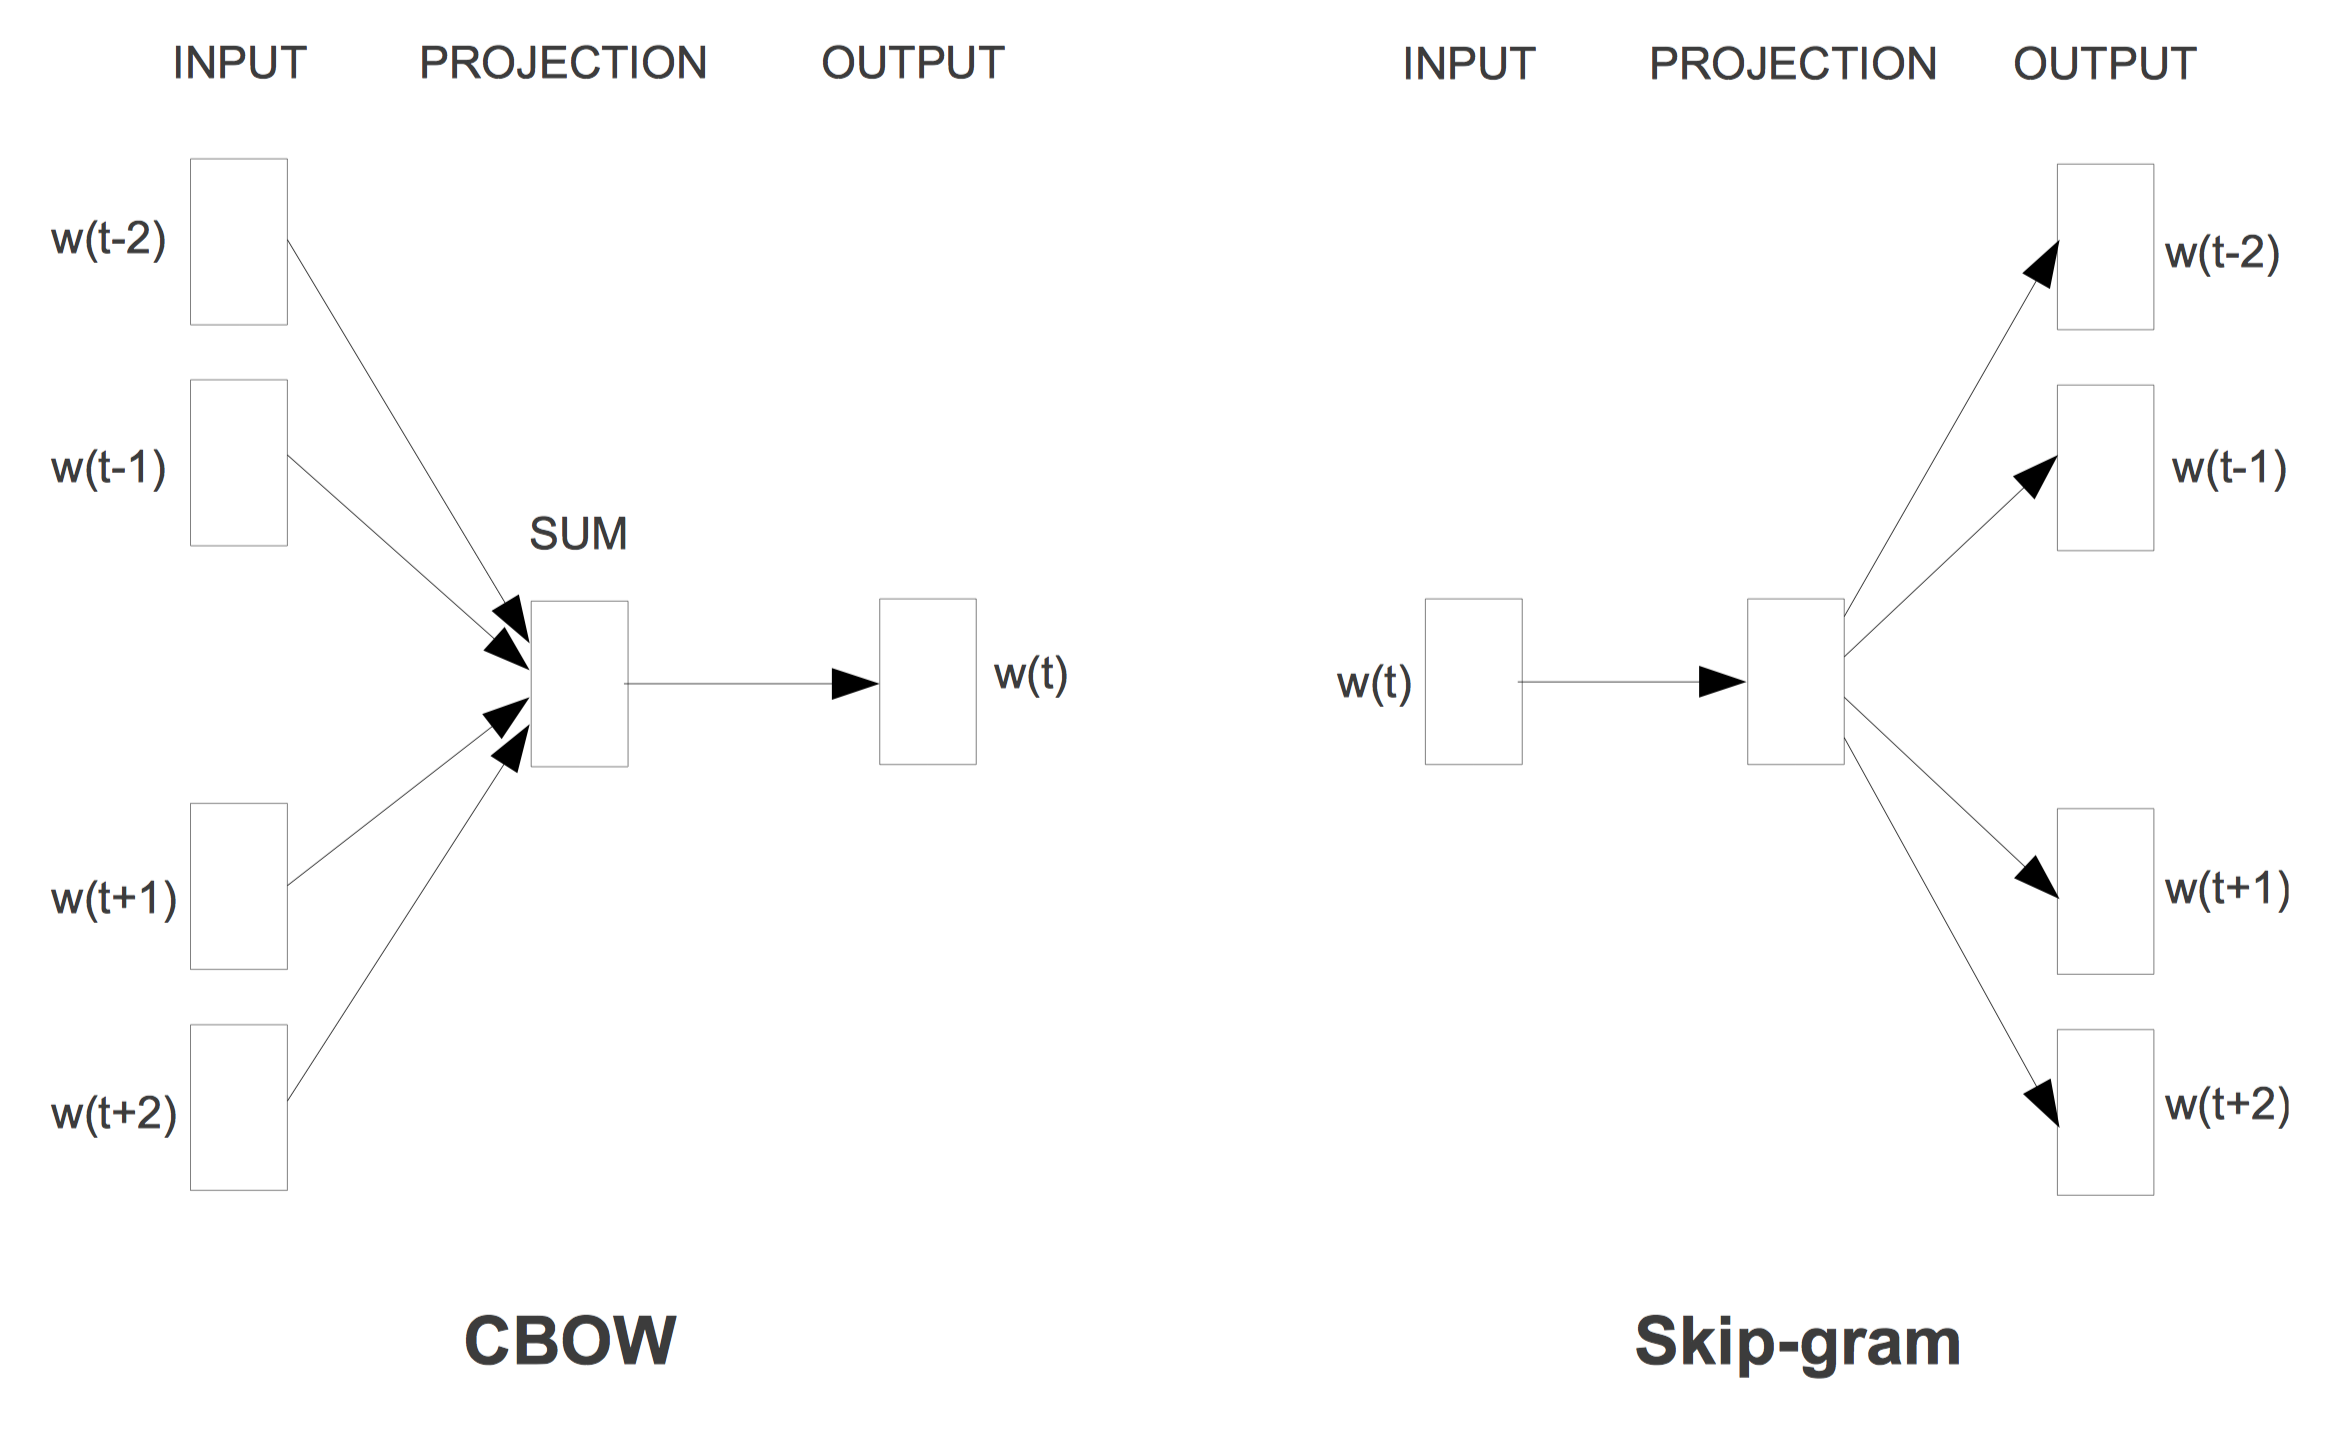
\includegraphics[width=0.7\textwidth]{./figures/cbow_vs_skipgram.png}
    \caption{The differences between the model architectures proposed by Mikolov in \cite{mikolov2013}. The Continuous Bag-Of-Words (CBOW) approach predicts a word from its context and, conversely, the skip-gram model predicts the context from a word. \cite{mikolov2013b}}
    \label{fig:cbow_vs_skipgram}
\end{figure}

Their work brought about a novel evaluation strategy which measures the expressive capacity of a word vector space through complex multi-dimensional comparisons that went over and above previous scalar metrics that were typically limited to the distance or angle between word vectors. As evidence of the level of sophistication obtained in the representations that were generated using the \textit{skip-gram} model, the authors note that the composition of vectors for words such as \enquote{Germany} and \enquote{capital} results in a vector that closely resembles the word \enquote{Berlin}. Additionally, more sophisticated linear translations could be modeled such as \enquote{Madrid} - \enquote{Spain} + \enquote{France} is resulting in a word vector closest to that of the word \enquote{Paris} \cite{mikolov2013c}.

While the skip-gram model required no dense matrix multiplications which made it substantially more efficient than most of the neural network implementations that had preceded it, in their experiments they note that the quality of the resultant word vectors could be improved by increasing the window size, however this would carry with it a corresponding increase in computational complexity. Nevertheless, \cite{mikolov2013} demonstrated that sufficiently expressive vector representations of words could be obtained from large corpora of data without the need for computationally expensive models.

Following their initial work, \cite{mikolov2013b} later expanded on their \textit{word2vec} models, introducing the negative sampling algorithm to improve the efficiency by which the model learned word vectors while proposing a method for accounting for phrases through a simple data-driven approach whereby particular phrases composed of multiple words were treated as a singular token, and trained-for as such.

As noted by \cite{mikolov2013}, the performance of their models were contingent on a set of design choices, most critical of which include the training algorithm, vector size, sub-sampling rate and the size of the training window. They conclude that the optimal configuration for these parameters varies based on the task being tackled.

\subsection{How is GloVe different to Word2Vec?}
Using co-occurrence statistics to extract continuous representations of words within a large corpus of data has been explored in NLP in works as early as \cite{rumelhart1988}, as cited by \cite{bojanowski2017}

\cite{pennington} argue that while the significance of word occurrence information within a text when learning word representations in an unsupervised manner is uncontested, further research is needed into the mechanisms by which these statistical data generate meaningful vector representations. In pursuit of this, they propose the \textit{GloVe} model, characterized by its use of the global, that is to say at the level of the corpus in its entirety, co-occurrence information to produce aptly-called \textit{\enquote{global vectors}}.

\cite{pennington} point out that while count and prediction based methods are not fundamentally dissimilar, since both exploit co-occurrence statistics within a corpus to obtain accurate representations, they argue for the efficiency of the former approach over the latter. 

A word-word co-occurrence matrix $X$ is constructed from a vocabulary such that $X_{ij}$ is representative of the number of times word $j$ is found in the context of word $i$. This invariably makes $X$ sparse in nature, since the substantial portion of words within a language cannot be expected to occur within an equally substantial number of words. 

\cite{pennington} develop \textit{GloVe} by only considering non-zero elements of the co-occurrence matrix of the corpus as a whole and as opposed to the sparse matrix in its entirety. This provides a substantial increase in speed and moreover, as their work suggests, generates more expressive representations of each word when compared to a limited window-based approach. \textit{GloVe} was evaluated on three separate tasks, specifically word analogy, word similarity and entity recognition tasks, achieving superior results over the previous literature in all. \cite{pennington}

Furthering the case for the capacity of the \textit{GloVe} model, the comparative study carried out on the task of reading comprehension by \cite{bhuwandhingra2017} demonstrated that pre-trained \textit{GloVe} embeddings outclassed other embeddings, including \textit{word2vec} \cite{mikolov2013}. From their experiments, \cite{bhuwandhingra2017} continue to suggest that these embeddings, in their off-the-shelf format, also surpassed embeddings trained on the target text itself as well as, to their surprise, an expanded corpus of data extracted from a domain commensurate with that of the target text.

\subsection{How is \textit{fasttext} different?}
Both \textit{word2vec} and \textit{GloVe} are considered as models operating on a word-level by regarding the word as the atomic operand, however \cite{bojanowski2017} argue that this approach is possibly sub-optimal when considering languages, such as Turkish and Finnish, where single words can have multiple morphologies, or comprise of exceedingly large vocabularies, or both. In contrast, they argue that the use of sub-word information lends itself well to these languages where the multiple morphologies of a word follow some form structure, such as specific verb conjugations. 

To tackle this issue they extend the \textit{word2vec} skip-gram model to operate at a sub-word level, adopting a bag-of-characters n-grams approach for word representation. As opposed to having each word represented by a vector, a word is represented as the aggregate sum of its constituent character n-grams. 

The authors also demonstrate how a vector for an OOV word can be constructed from its character n-grams with remarkable similarity to a comparable IV word. Some of their results can be seen in \ref{fig:fasttext_oov_similarity}, where an OOV word \enquote{microcircuit} shows positive cosine similarity (in red) to an IV word \enquote{chip} between its constituent character n-grams \enquote{micro} and \enquote{circuit}.

\begin{figure}[!ht]
    \centering
    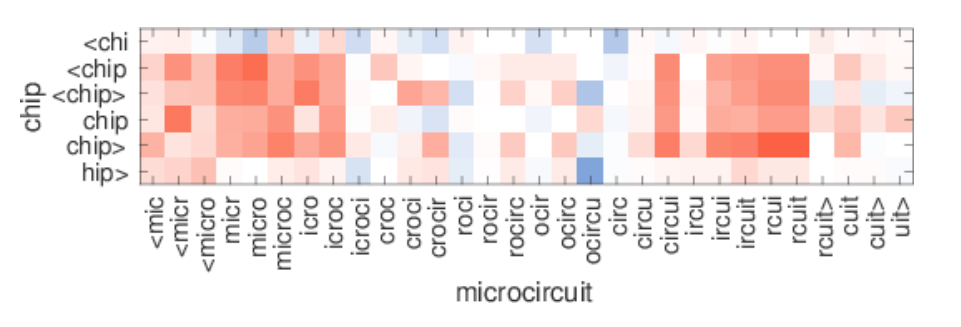
\includegraphics[width=0.7\textwidth]{./figures/fasttext_oov_similarity.png}
    \caption{Character n-gram similarity between the OOV word \enquote{microcircuit} and IV word \enquote{chip}. Positive and negative cosine similarity are denoted in red and blue respectively. Figure adapted from \cite{bojanowski2017}}
    \label{fig:fasttext_oov_similarity}
\end{figure}

\textbf{Need to include disadvantages of fasttext to make a contrast}
%\cite{bojanowski2017} report excellent training times for their unsupervised approach, without the need for any pre-processing, while outperforming other benchmark models that do not make use of sub-word information or use techniques such as morphological analysis. 

\section{Deep Learning}
\subsection{What are the fundamentals of a Neural Network?}
Modelled on the human brain, neural networks typically involve a series of layers composed of neurons. Figure \ref{fig:ffnn} illustrates one such simplified neural network architecture with a single hidden layer, $L_2$, preceded by the input layer $L_1$, and followed by the output layer $L_3$. $(x_1, x_2, x_3)$ represents a three dimensional input vector, whereas the neurons, or hidden units, of the of the network are depicted as $(h_1, h_2, h_3)$. The firing action of each neuron is expressed using a non-linear activation function. This action propagates from one neuron in a layer to all other connected neurons in the subsequent layer and is modulated by a particular weight that characterizes each intra-neural connection. At minimum, these networks will incorporate an input and an output layer that will encapsulate one, or more, hidden layers. 

The network is able to learn, or model, a function by adjusting the weights to minimize a some measure of error towards a particular objective function. \cite{graves2012b}

The hidden layers of a neural network architecture are able to extrapolate features at a level that cannot be carried out manually, thereby capturing more subtle details and generating richer representations of the data being learned. Foregoing this need for extensive manual feature engineering is one of the primary drivers of neural network models, even though these are approaches are typically black-box solutions, with obfuscated inner-workings.
 
\begin{figure}[!ht]
    \centering
    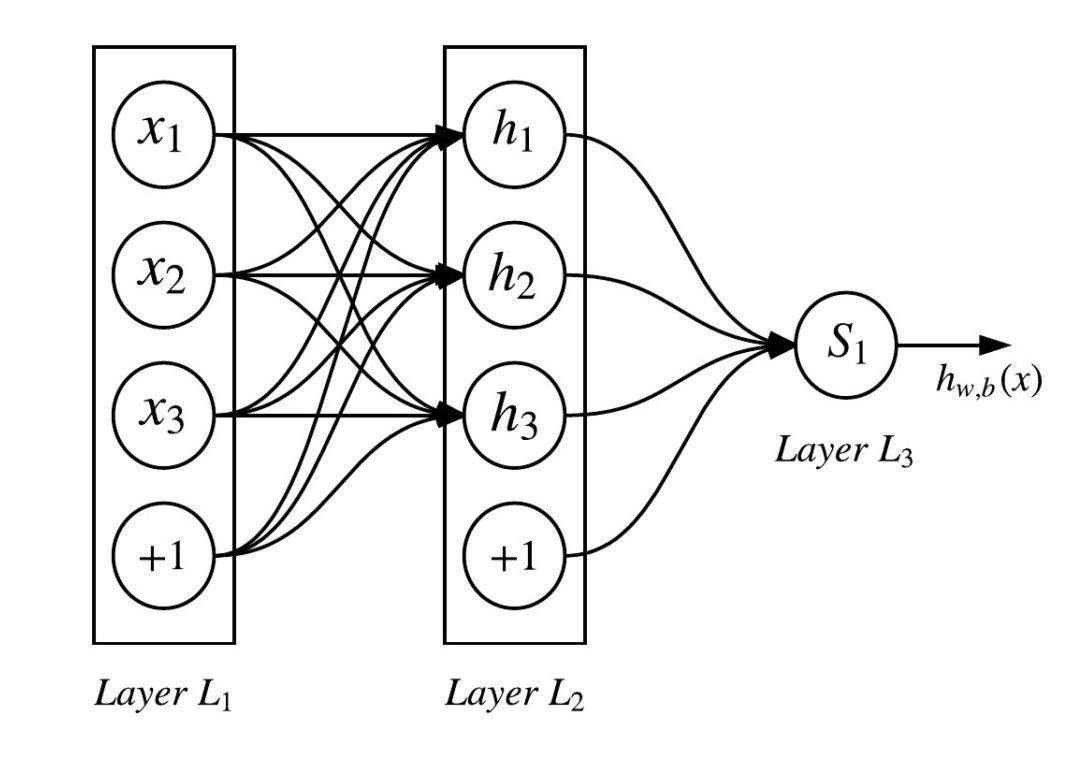
\includegraphics[width=0.7\textwidth]{./figures/ffnn.jpg}
    \caption{Standard feedforward neural network (FFNN) architecture \cite{zhang2018}}
    \label{fig:ffnn}
\end{figure}

\subsection{What are the common activation functions?}
Three of the most commonly used activation functions are sigmoid (eq. \ref{eq:sigmoid}), hyperbolic tangent (eq. \ref{eq:hyperbolic_tangent}) and Rectified Linear Unit (ReLU; eq. \ref{eq:relu}). Although the choice of activation function is typically heuristic, \cite{glorot2011} as cited in \cite{zhang2018} notes that the ReLU is easier to compute when compared to the other two and also tends to converge faster, all while maintaining similar or even better performance. 

\begin{equation} \label{eq:sigmoid}
    f(W^tx) = sigmoid(W^tx) = \frac{1}{1+e^{-W^tx}}
\end{equation}
\begin{equation} \label{eq:hyperbolic_tangent}
    f(W^tx) = \tanh(W^tx) = \frac{e^{W^tx}-e^{-W^tx}}{e^{W^tx}+e^{-W^tx}}
\end{equation}
\begin{equation} \label{eq:relu}
    f(W^tx) = ReLU(W^tx) = \max(0,W^tx)
\end{equation}

\subsection{How are Neural Networks typically trained?}
Neural networks are trained by following the direction of the gradient that lessens the measured error rate of some objective function which is calculated through the repeated application of the chain-rule. The process can be carried out on the training set in its entirety, commonly referred to as batch learning, or in an on-line manner, carrying out updates after each training sample. The latter is known as stochastic gradient descent and is known to be more efficient and robust to local minima when dealing with large datasets \cite{lecun1998} as cited in \cite{graves2012b}. 

There will always be noise in the sampled training data that does not translate to the real world test data scenarios and that the model must therefore avoid learning. Training models to the point of becoming overly-sensitive to this noise is referred to as over-fitting the data, and there are a number of regularization techniques often employed in the literature while training to counteract this. 

One common approach is introducing some form of weight penalties, for instance, $L1$ and $L2$ regularization. Other techniques frequently used include \textit{early-stopping}, whereby a fraction of the training data is used as a validation set that the model is tested against at regular intervals during training to test for a sustained improvement \cite{graves2012}, and \textit{dropout} \cite{srivastava2014}, in which random neurons in a NN are ignored (\enquote{dropped}) with some probability $p$, effectively training a diverse range of \enquote{thinned} versions of the original NN. An approximated average of those networks is subsequently used as final trained model by scaling its weights by that same dropout probability $p$. 

\subsection{How are Deep Neural Networks formed?}
\enquote{Deep} neural networks are constructed by stacking a series of layers in such a way that salient features extracted from one layer are passed on as input data to the next layer, and so on. This stacking process, in theory, improves the capacity of the network to extract more abstract and expressive features that reside at a deeper level within the input data. \cite{zhang2018}  

\subsection{Why is Deep Learning popular again recently?}
In recent years, the astounding progress in computing resources such as GPUs and high performance distributed computing have made deep learning accessible on an unparalleled level. Consequently, this has driven interest in the applicability of deep learning architectures such as the CNN and RNN in a range of fields from computer vision to natural language processing \cite{goldberg2015}, \cite{collobert2011}.

\subsection{What are two common deep learning models used? (CNN and RNN)}
Not least owing to their impeccable ability for effectively extracting highly expressive low-dimensional representations of text automatically, coupled with the aforementioned resurgence of deep learning due to the increase in available computing power, the use of neural network models such as \cite{lakkaraju2014} \cite{vo2015} \cite{nguyen2015}  became increasingly widespread within the field of NLP, including targeted and aspect based sentiment classification tasks \cite{dong}; \cite{wang}; \cite{tang2016} \cite{tang2016b}.

The most prevalent architectures are the Convolutional Neural Networks (CNNs) and Recurrent Neural Networks (RNN) and the descendents thereof. Other deep learning models worth mentioning include the Recursive Neural Network (Rec-NN), which has been employed in works such as \cite{socher2011} and \cite{socher2013} for syntactic analysis and sentence sentiment analysis respectively. \cite{zhang2018}

\subsection{What are the fundamentals of a CNN (in brief)?}
The layers typically comprise of filters, also referred to as kernels, of differing widths that slide over the input data to extrapolate various features. Each of these features would be representative of a diverse set of aspects of the data that would aid in defining it with respect to the task being tackled.  

These convolution layers are coupled with a max-pooling layer with the intention of extracting the most salient values. These values can subsequently be forwarded to another convolution layer that presumably extrapolates deeper, more abstract features. This process can be repeated a number of times across multiple convolution layers to build a deep CNN that eventually produces a single feature vector representation of the original input data. Figure \ref{fig:cnn_architecture} illustrates this process using six filters with three difference widths and two diverse operations for each, the results of which are down-scaled using max-pooling, and subsequently passed through a softmax function for binary classification. 

\begin{figure}[!ht]
    \centering
    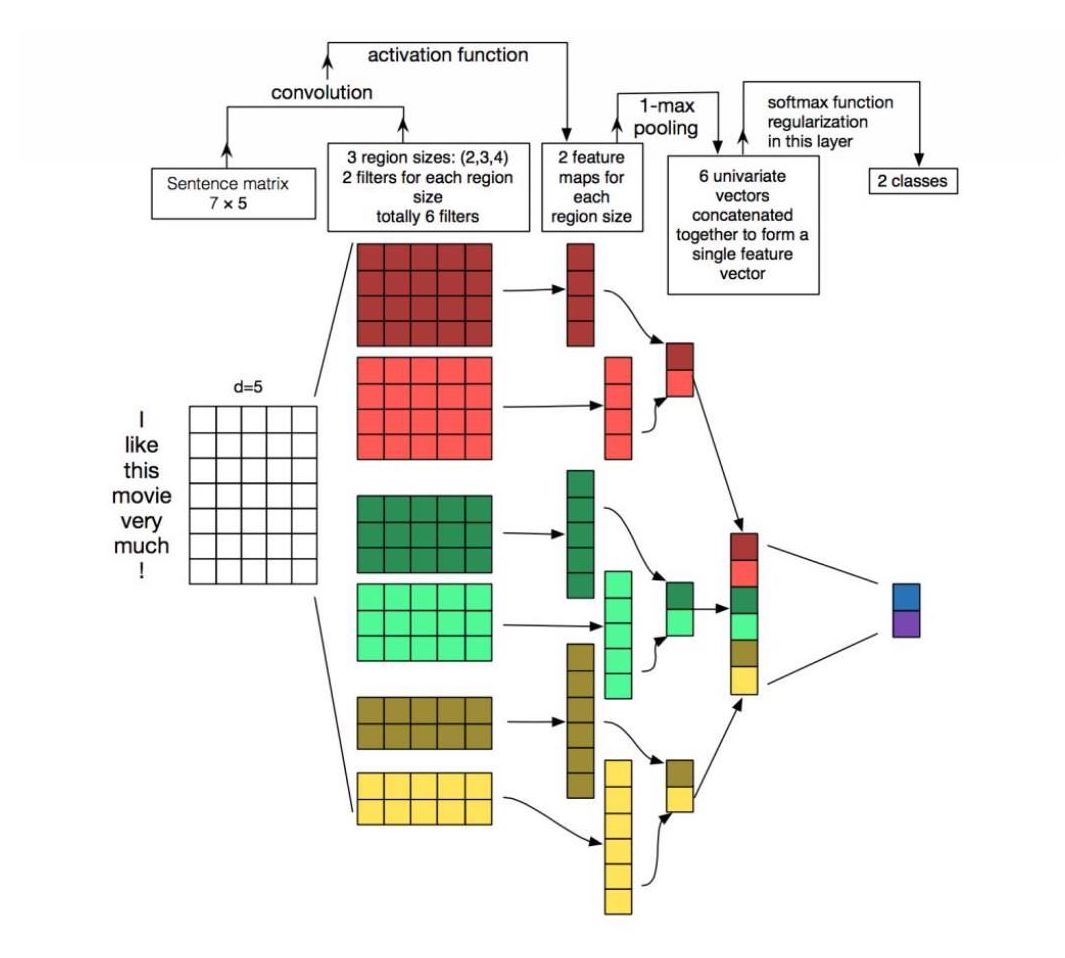
\includegraphics[width=0.7\textwidth]{./figures/cnn_architecture.jpg}
    \caption{An example of a CNN architecture used for sentence modelling and subsequent binary classification \cite{yezhang2015} as cited in \cite{young2017}.}
    \label{fig:cnn_architecture}
\end{figure}

\subsection{What are the advantages of using max-pooling?}
Max-pooling is ideal for producing a fixed-length representation of the data, which is a common prerequisite for classification tasks, while at the same time preserving the most prominent features from the original data. \cite{young2017}

\subsection{What are some approaches using CNN?}
Some of the first CNN-based approaches that paved the way for the growth of CNN architectures in the literature that followed were \cite{collobert2011}, \cite{kim}, and \cite{kalchbrenner2014}.
\cite{kim} used CNN architecture for sentence classification tasks ranging from subjectivity and question type with promising results albeit in the face of a number of challenges that became evident to the authors. Not least of these was the limited capacity for the CNN architecture to capture syntactical dependencies in sentences that occurred over long distances. This challenge was the one of the foremost drivers for the work that followed by \cite{kalchbrenner2014} who developed the DynamicCNN (DCNN) which consisted of a series of hierarchical convolution and k-max pooling layers.

Other works cited in \cite{young2017} include \cite{poria2016} that dealt with sarcasm detection on twitter data, noting a need for additional context information when dealing with short texts of this nature. This observation is also echoed in \cite{johnsonzhang2015}, who noted superior performance of CNN networks when dealing with longer text that would provide more contextual information as opposed to shorter text. Due to the vast amount of parameters that CNNs typically need to learn, scarcity of data is an often cited challenge \cite{young2017}.

Work carried out by \cite{chen2016} made use of a CNN to deduce the sentiment of the target based on the sentiment of the clause surrounding it. As noted by \cite{chen2017} however, this method still operated on the assumption that the most salient features of a word can be extracted from other words in close proximity.

A phrase such as \enquote{I bought a mobile phone, its camera is wonderful but the battery life is short, not particularly satisfied overall}, challenges this assumption with respect to the \enquote{mobile phone}, as the intended target since the most sentimentally-laden words appear at the opposite end of the sentence.  

\subsection{What are the fundamentals of an RNN based model (in brief)?}
A Recurrent Neural Network (RNN) can be thought of as a chain of recurring modules which typically represent elements within a variable-length sequence, with an internal hidden state that represents the network's \enquote{memory}. This state is passed forward from one module in the chain to the next.

Unlike a CNN, where each layer has its own set of trainable parameters that must be learned, a RNN uses a single set of parameters across all of the modules in the chain which significantly diminishes the total number of parameters that it must learn.

Through forwarding the hidden state from one time step in the chain to the next, the network is able to \enquote{remember} information from previous elements of the sequence and use that information when generating a representation for the current element \cite{tang2016b}. 

\subsection{What makes the RNN more suitable for targeted sentiment analysis? (sequence)}
The hidden state that characterizes RNNs acts as its \enquote{memory} element and makes these networks particularly effective in dealing with data that are sequential in nature. One of the most prominent examples of these data is language, where the significance of a word at one time step may be substantially altered by those that preceded it. Consider, for example, the word \enquote{dog}, for which the meaning would shift entirely, from an animal to a popular American snack, should it be preceded by the word \enquote{hot} \cite{young2017}.

Moreover, the capacity of RNNs to model variable length sequences to a fixed length representation also makes them particularly practical when dealing with different units of resolution in languages including documents, sentences, and even words, all of which are naturally arbitrary in length. \cite{tang} 

\subsection{What is problem faced by RNN? (vanishing \& exploding gradient)}
In the setting of a traditional RNN, the tendency for a gradient to exhibit exponential change to the degree that prevents substantive learning increases with the length of a sequence \cite{bengio1994} \cite{hochreiter1997}. This phenomenon is what is implied by the terms \enquote{vanishing} or \enquote{exploding} gradients, where the changes observed over time steps often vanish with time or, although less frequently, but with equally devastating results, grow exponentially; hindering the network's capacity for learning.

\subsection{What solutions exist to  vanishing/exploding gradient problem? (LSTM and GRU)}
One class of solutions to the vanishing or exploding gradient problem is to carry out particular modifications on top of the standard stochastic gradient descent algorithm, such as gradient clipping, whereby the norm of the gradient vector is \textit{clipped}, or using second order derivatives, which may or may not be influences to a lesser degree. \cite{chung2014}
The second, and more popular, class of solutions look instead to introduce further sophisticated, additive, non-linearities to the traditional RNN unit. These would selectively carry forward salient features and filter out irrelevant information from previous time steps, as opposed to overwriting the memory content at each time step.  

Variants on the standard RNN network were proposed to address the vanishing and exploding gradient issue. The most popular of these being the Long Short Term Memory (LSTM) and, more recently, Gated Recurrent Unit (GRU). Other approaches include, but are not limited to, Residual Networks (Res-Net).

\subsection{What are the fundamentals of the LSTM (in brief)?}
LSTM \cite{hochreiter1997} is an extension on the RNN model that addresses the issue of a vanishing or exploding gradients through the use of gates that control the flow of information from the past states to present states.

To do this, the LSTM introduces three adaptive gates that can be considered additional neural layers on top of the single neural layer that characterizes the typical RNN. The layers introduce an increased level of sophistication in the \enquote{remembering} process from one sequence point to the next.

These gates are commonly referred to as the input, forget and output gate. Moreover the LSTM also maintains a two inner states as opposed to one, namely the cell state and the hidden state.

\begin{figure}[!ht]
    \centering
    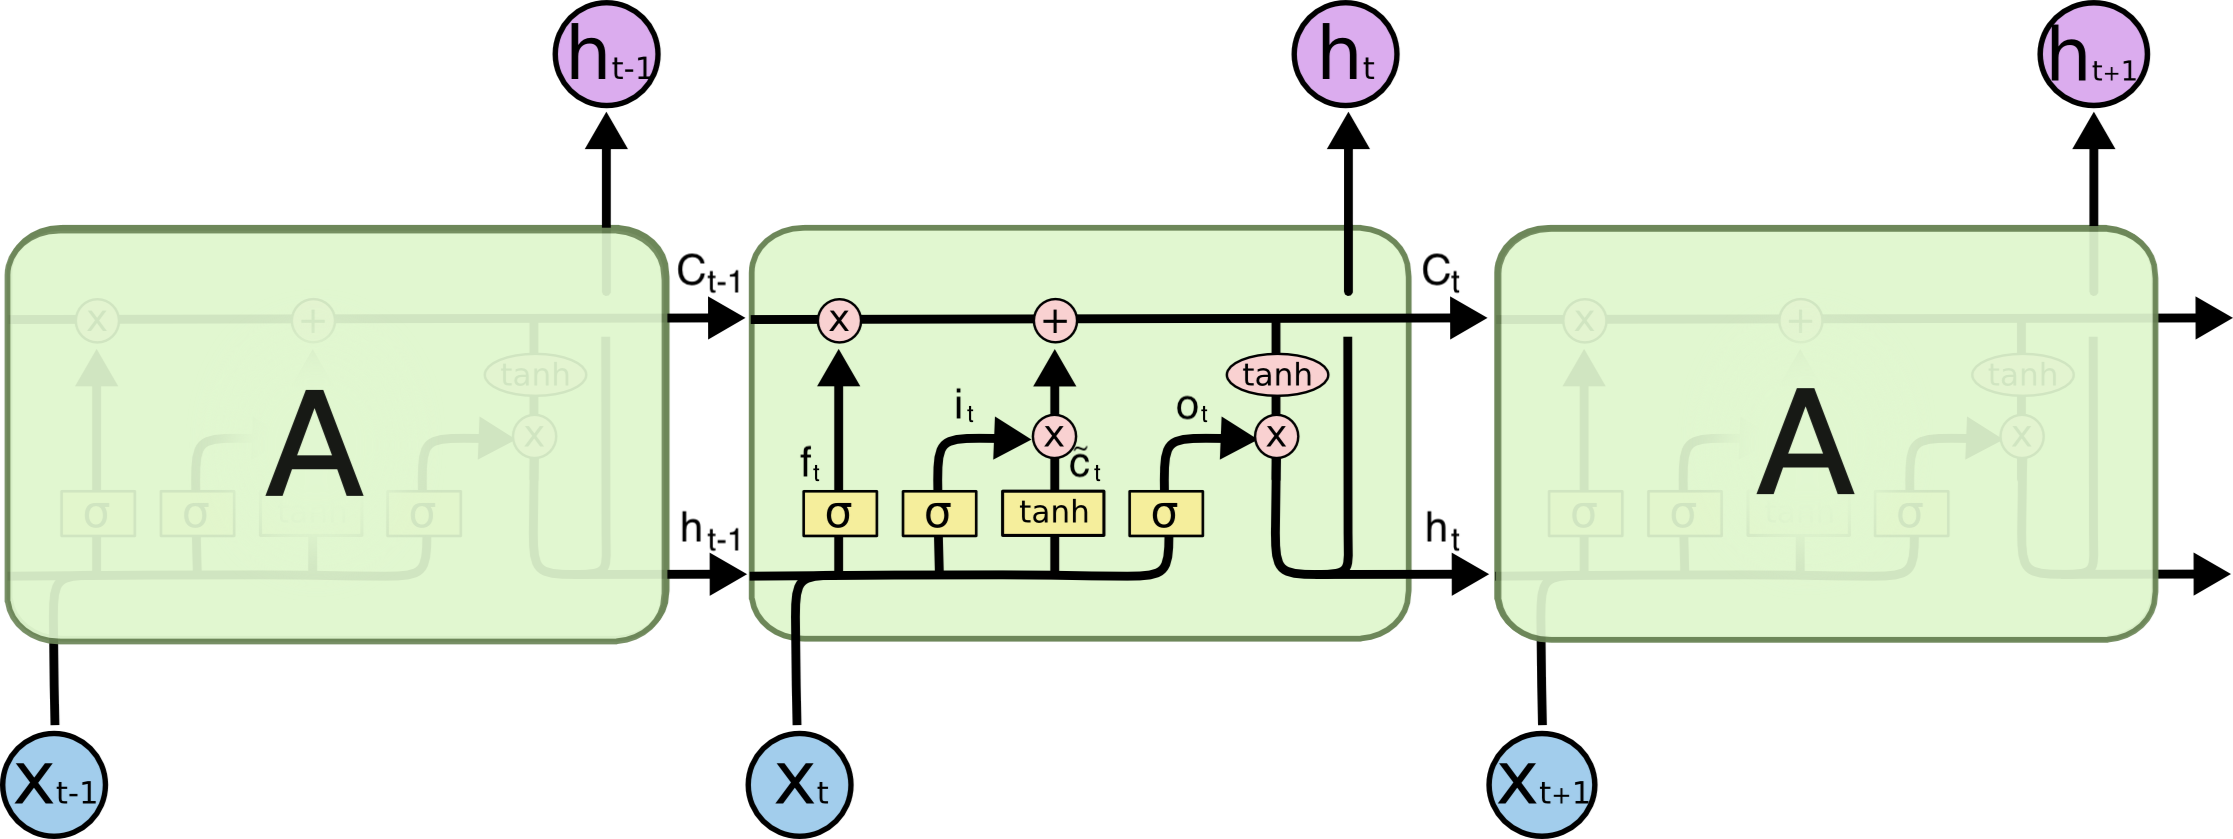
\includegraphics[width=1\textwidth]{./figures/lstm_architecture.png}
    \caption{LSTM repeating module illustrating the four neural layers (Yellow Boxes) that comprise it. Point-wise vector operations are depicted in red boxes. Image adapted from \cite{colah-understanding-lstm}}
    \label{fig:lstm_architecture}
\end{figure}

The process undergone in each repeating module of the standard LSTM architecture depicted in figure \ref{fig:lstm_architecture} starts at the forget gate. Here, the information to be removed from the cell state $C_{t-1}$ is selected through the sigmoid layer (eq. \ref{eq:lstm_forget_gate}). 
\begin{equation} \label{eq:lstm_forget_gate}
    f_t = \sigma(W_f\cdot[h_{t-1},x_t] + b_f)
\end{equation}
Next, an update vector is produced through a point-wise multiplication operation between the input gate (\ref{eq:lstm_input_gate}), which represents the values selected to be updated, and a vector of candidate values, $\Tilde{C}$ (\ref{eq:lstm_candidate_cell}). This update vector is added to the current cell state, from which the forget gate had previously removed information deemed redundant. 
\begin{equation} \label{eq:lstm_input_gate}
    i_t = \sigma(W_i\cdot[h_{t-1},x_t] + b_i)
\end{equation}
\begin{equation} \label{eq:lstm_candidate_cell}
   \Tilde{C} = \tanh(W_C\cdot[h_{t-1},x_t] + b_C)
\end{equation}
Finally, an output gate (\ref{eq:lstm_output_gate}) regulates the amount of cell state information that is output to the rest of the network through the unit's hidden state $h_t$ (eq. \ref{eq:lstm_hidden_state}). 
\begin{equation} \label{eq:lstm_output_gate}
    o_t = \sigma(W_o\cdot[h_{t-1},x_t] + b_o)
\end{equation}
\begin{equation} \label{eq:lstm_hidden_state}
    h_t = o_t*\tanh(C_t)
\end{equation}

\subsection{How does the LSTM model address the  vanishing \& exploding gradient problem?}
The gating mechanism that is present in the LSTM network allows for the persistence of salient features that are encountered early in the sequence and which would otherwise be overwritten in a typical RNN architecture.

The input and output gates of the LSTM control the amount of memory content that is to be added to the memory cell and the memory content that is exposed to the rest of the network respectively.

Forget gates were later added to the architecture \cite{gers2000}, which enabled the memory cells to reset themselves. It is important to note that the LSTM updates the memory cell independently from the forget gate, which is to say that, for the LSTM to \enquote{remember} a prior input in a sequence two conditions must be satisfied; the input gate must be closed, preventing the addition of new information and, the forget gate must be maintained open, as otherwise this would cause the existing memory content to be reset.

\subsection{What are some approaches using LSTM?}
\cite{wang} achieved results competitive with those obtained by \cite{kalchbrenner2014} by using an LSTM, as opposed to CNN, to generate representations of tweets. \cite{young2017} notes that their model was able to extract features over long distances at a fraction of the complexity of the DynamicCNN \cite{kalchbrenner2014}.

Another variant on the LSTM architecture involved the use of dependency parsing to build tree-structured LSTMs which operate on some specific tree-pattern that is extracted from the data, typically through the use of external parsing tools \cite{socher2013}. Approaches of this variety \cite{jiweili2015}, \cite{kaishengtai2015}, \cite{zhu2015} have obtained promising results, however as \cite{chen2017} note, these are contingent on the data being well-formed structurally and grammatically, which is not guaranteed when dealing with micro-texts on social media platforms.

Two of the foremost extensions on the classical LSTM model when tackling target-based sentiment analysis, were proposed in \cite{tang2016b} with the intent of accounting for the target information, these were termed the Target Dependent LSTM (TD-LSTM) and Target Connection LSTM (TC-LSTM). Their work showed that the changes proposed would improve the performance over a standard LSTM. \cite{tang2016b} generate representations of a target's left and right contexts, where the target representation is concatenated to each. These two are then finally chained together to form the final, target-specific, representation of the sentence which is fed to an LSTM for sentiment classification \cite{dehongma2017}.

TC-LSTM \cite{tang2016b} was reported as one of the first neural network based methods to obtain state-of-the-art performance without the use of laborious feature engineering and external data sources. It is worth noting however that recent work \cite{moore2018} failed to reproduce the original results that were reported.

\subsection{What are difficulties mentioned that LSTMs deal with?}
While the issue of long-distance dependencies and CNN based approaches is often brought up, \cite{chen2017} remarks that LSTMs will still struggle with features that are located too far apart within a sequence, given the phrase \enquote{Except Patrick, all other actors don’t play well}, an LSTM would struggle to identify the positive sentiment on the opinion target \enquote{Patrick} due to the distance between the terms \enquote{Except} and \enquote{don't play well}.

From the observation made by \cite{bahdanau2014} when employing LSTM-based models in the field of machine translation, \cite{chen2017} make the case that the TD-LSTM would suffer from in instances where the most sentimentally salient word is located further away from the target being considered. 

\subsection{How does a Bi-LSTM differ from an LSTM?}
When dealing with bounded sequences, a natural conclusion one  might draw is that valuable information can be extrapolated from future contexts as well as past contexts. Bidirectional RNNs are employed with this specific intention in mind. 

Building on top of the LSTM architecture, a Bi-LSTM is so called as it is the result of two stacked LSTMs, each responsible for processing and extracting features from a sequence in opposite directions. Features extracted from these two directions are then typically concatenated into a single, theoretically richer, and more expressive, representation of the sequential data.

It has been argued that the bidirectional nature of these models violates causality, which is justified to an extent, since a future context cannot be exploited if it is the same element that is being predicted. An example of this is predicting future stock market fluctuations. However, for tasks where this information is available, bidirectional variants that make use of this information have consistently been shown to outperform their uni-directional counterparts. \cite{graves2012b} 

\subsection{What are some approaches using Bi-LSTM?}
Sentence and document level sentiment classification tasks lend themselves well to the use of bi-directional RNN (BRNN) variants, since the boundaries of the sequence being classified are well-defined a priori. In their work, \cite{chen2017} suggest that using a BLSTM improves the ability of their approach to extrapolate phrase-like features when compared to a uni-directional sequential approach. 

An improvement in results stemming, in part, from taking a bi-directional approach is also observed in \cite{zhang2016}, in both accuracy and macro F1 scores when compared to the work of \cite{vo2015}, from which the former was inspired. More recent works (eg. \cite{ma2018}, \cite{zheng2018}) that have reported notable results in the field also take advantage of bi-directionality in their approach. 

\subsection{What are the fundamentals of the GRU (in brief)?}
The GRU does away with the cell state that is found in the LSTM, maintaining only a single hidden state as its \enquote{memory}. The second way in which the GRU differs from the LSTM is in its number of gating units, by foregoing the output gate and combining the input and forget gates into a single update gate, the GRU benefits from having less parameters to learn.
\begin{equation} \label{eq:gru_update_gate}
    z_t = \sigma(W_z\cdot[h_{t-1},x_t] + b_z)
\end{equation}
As the name implies, when the reset gate (eq. \ref{eq:gru_reset_gate}) nears $0$, it allows the GRU unit to drop the previous information, which may be deemed inconsequential at a later time, and reset itself with the current input only. This information is then used by the GRU to produce a vector of candidate activation values (eq. \ref{eq:gru_candidate_activation}).
\begin{equation} \label{eq:gru_reset_gate}
    r_t = \sigma(W_r\cdot[h_{t-1},x_t] + b_r)
\end{equation}
\begin{equation} \label{eq:gru_candidate_activation}
    \Tilde{h}_t = \tanh(W\cdot[r_t * h_{t-1},x_t] + b)
\end{equation}

Instead of maintaining an internal memory cell, the GRU uses the update gate and carries out a linear interpolation function (eq. \ref{eq:gru_update_interpolation}) to control the amount of candidate activation, $\Tilde{h}_t$, that is added to the previous activation. In this way the update gate serves as the primary mechanism preventing the GRU from overwriting a previously encountered salient feature. 
\begin{equation} \label{eq:gru_update_interpolation}
    h_t = (1-z_t)*h_{t-1} + z_t*\Tilde{h}_t
\end{equation}
Whereas the LSTM utilizes the output gate to control the exposure of its internal memory to the rest of the network, the GRU does not have any means by which to control the exposure of its inner state, and therefore exposes its hidden state in its entirety to the rest of the network.  

Each unit in a GRU model will have separate update and reset gates that will independently learn to capture long and short term dependencies in a sequence. Units that learn to capture longer-term dependencies will have active update gates whereas, for short-term dependencies, the reset gates will tend to be more active.

\begin{figure}[!ht]
    \centering
    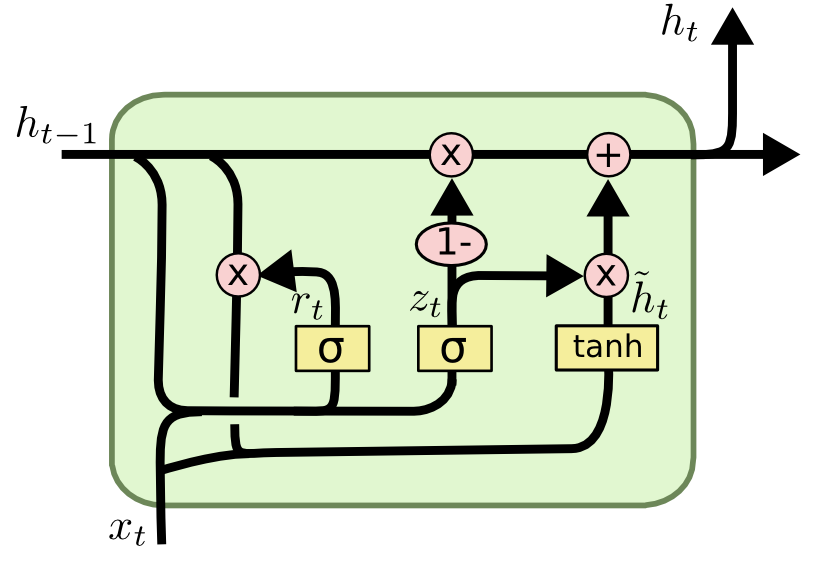
\includegraphics[width=0.7\textwidth]{./figures/gru_architecture.png}
    \caption{Internal gating structure of a GRU unit. \cite{colah-understanding-lstm}}
    \label{fig:gru_architecture}
\end{figure}

\subsection{What are some approaches using GRU?}
\cite{zhang2016} model the interplay between targets and their contexts through gated mechanism operating on the a representation of the original sentence split into three components using a gated-RNN.  

\cite{liu2018} use a GRU as part of their approach, serving as a gating mechanism to determine whether to update a specific part of memory based on past activations. They claim state of the art results in aspect detection and sentiment classification, outperforming SenticNet \cite{ma2018}, and foregoing the need of external knowledge.

\cite{xue2018} use gated tanh-ReLU units to control flow of features from convolutional neural networks to max pooling layer. They deal more with the advantages that a CNN offers, since it is not time-dependent and is therefore easier to parallelize. 

\cite{jabreel2017} generate a sentence representation by stacking two GRU based networks, similar to the BLSTM configuration, opting to go with the GRU architecture instead since it has less parameters to learn, noting similar results. A continuous vector representation of the target is sandwiched between the two GRU direction outputs, and fed to softmax classifier. Authors report accuracy and macro-f1 scores better than state of the art obtained on a twitter dataset \cite{dong}.

\subsection{What advantages/disadvantages does the GRU have over the LSTM if any?}
Since the architecture of the GRU is less complex than that of the LSTM, there may be circumstances where the former may be more efficient than the latter since it requires less parameters to learn \cite{chen2017}, \cite{jabreel2017}.

That being said, there is no clear winner between the two variants, as demonstrated by work conducted in \cite{chung2014}. The results obtained, shown in figure \ref{fig:rnn_v_lstm_v_gru_graphs}, concluded that the only demonstrable advantage is that of both variants over a standard RNN architecture. The authors go on to say that the performance of the two variants themselves is contingent on the particular nature of the tasks being addressed. Although it is worth noting that the work carried out by \cite{chung2014} was not specifically in the field of NLP, the deciding factor between these variants in NLP literature still tends to be heuristic \cite{young2017}.

\begin{figure}[!ht]
    \centering
    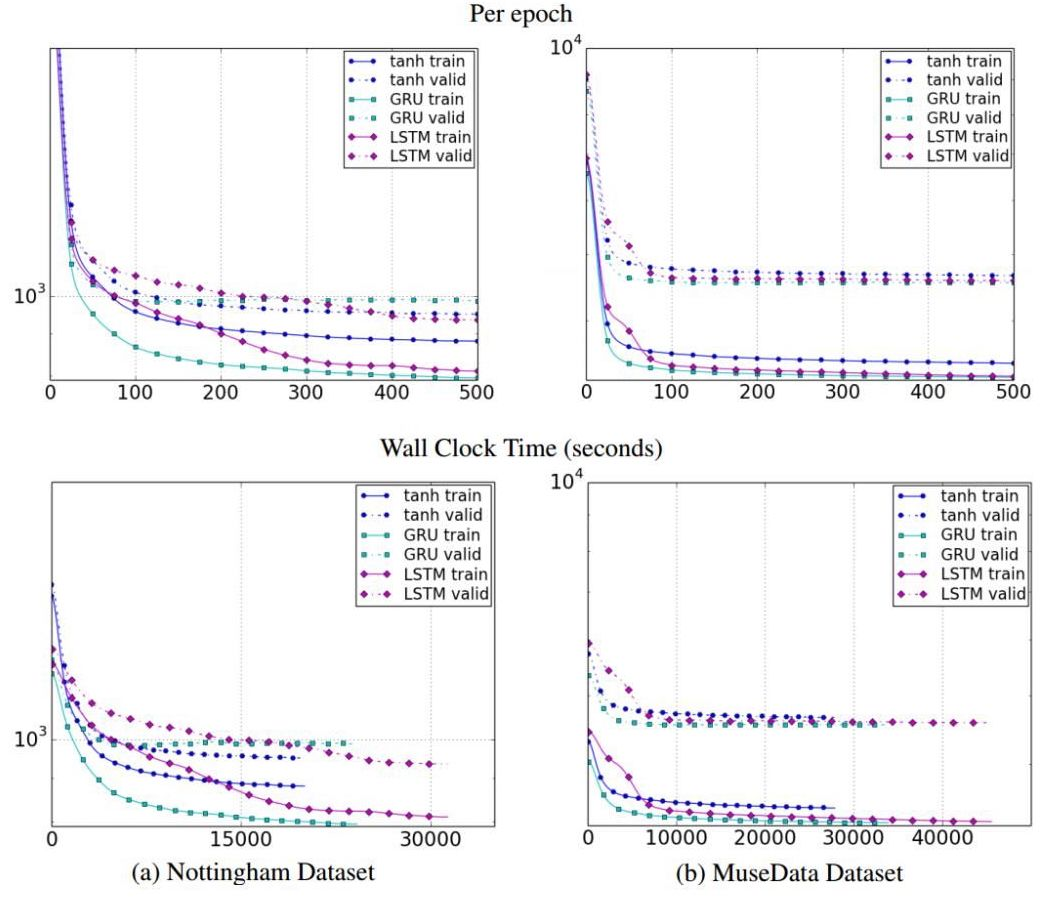
\includegraphics[width=0.7\textwidth]{./figures/rnn_v_lstm_v_gru_graphs.jpg}
    \caption{Results obtained by \cite{chung2014} during training and validation of different RNN variants illustrating the superiority of LSTM and GRU units over the traditional RNN.}
    \label{fig:rnn_v_lstm_v_gru_graphs}
\end{figure}

\subsection{Are there any advantages of CNN over RNN models?}
In spite of various studies illustrating the fact that CNN networks are data heavy in nature and often require auxiliary data when dealing with micro-texts such as those obtained from social media networks such as twitter, \cite{young2017} note that assuming the superiority of RNNs for sequential data is inaccurate.

They proceed to cite studies where CNNs performed competitively, and even surpassed RNN-based architectures in tasks for which the latter would, in theory, be better suited, such as language-modelling \cite{dauphin2017} as cited in \cite{young2017}.

It is worth keeping in mind that when dealing with language modelling, RNNs and CNNs approach the task from separate avenues; while RNNs, and their descendents, have no context boundaries when processing sequential data to generate a representation, CNN-based approaches seek to extrapolate the most meaningful n-grams from bounded-contexts from that sequence, to produce their final representation. \cite{young2017}

\subsection{Are there any approaches that use both CNN and RNN models?}
There have been works in the field of sentiment analysis, targeted and otherwise, with the intention of taking advantage of the benefits of both CNN and RNN based models in an ensemble approach. \textit{Finki} \cite{stojanovski2016} and \textit{BB\_twtr} \cite{cliche2017} are two solutions of this nature, dealing with sentiment analysis of tweets. These models involve the coupling of LSTM or GRU models with CNN models to carry out both binary, and fine-grained (five degrees) sentiment analysis on tweets. The works were part of the submission made to the yearly SemEval conference, and each performed impressively in their respective rounds.

While \cite{stojanovski2016} and \cite{cliche2017} were not addressing \textit{targeted} sentiment analysis, recent works such as \cite{xue2018} and \cite{xinli2018} also marry GRU or BLSTM with CNN models. Interestingly, both works cite the simplicity of their approaches when compared to more complex attention mechanisms as a driving factor, while still achieving comparable results in their experiments.  

\subsection{What does an attention mechanism seek to model?}
The intuition behind an attention mechanism is that, when dealing with sequential data, different parts of the sequence contribute to varying degrees towards a specific task or goal. This is abundantly apparent in the field of machine translation, where the attention mechanism made its debut \cite{bahdanau2014}  

When translating a particularly long sequence, for example, it is natural to focus principally on specific regions related to the current element being translated, as opposed to the source sentence as a whole, as this would result in the most relevant parts possibly being shadowed by unrelated material. 

\subsection{Where was attention first applied?}
The remarkable power of attention mechanisms for machine translation \cite{bahdanau2014} sparked an interest in investigating their applicability in a range of other tasks, including target, and aspect, based sentiment analysis \cite{wang} \cite{chen2017} \cite{dehongma2017} \cite{zheng2018}, image captioning \cite{kelvinxu2015} and question answering \cite{hermann2015}, where the notion of the most salient features being dispersed unevenly across the source data also holds true. 

\subsection{What are the fundamentals of the standard attention mechanism?}
In its simplest form, an attention mechanism involves a layer which produces a weight vector that represents a distribution of salience across an original feature vector, which would otherwise be considered evenly in its entirety, with respect to some target. The nature of the target varies depending on the downstream task, in targeted or aspect based sentiment analysis this is typically the target or aspect in question, whereas in fields such as machine translation this could be the last hidden state that was output.   

This process typically takes the form of some scoring function, such as a simple FFNN, which can be trained alongside the rest of the model, followed by a softmax layer. Given a series of representations $[h_{1}, h_{2}, ..., h_{n}]$ and some target $t$, the scoring function $a$ calculates the salience of each $h_{i}$ with respect to $t$. Subsequently, the softmax layer squashes the attentions scores into a valid distribution vector $\alpha$ with values in the range $(0, 1)$. 

\begin{equation} \label{eq:attention_alignment_model}
    \alpha_{i} = \frac{\exp(a(h^{i},t))}{\sum_{j=1}^{n}\exp(a(h^{j},t))}
\end{equation}

This weight vector is then used to produce a context vector $c$, as the weighted sum of the original feature vector. This process will amplify features with high attention weight values (approaching 1) while attenuating features with low attention weight values (approaching 0).

\begin{equation} \label{eq:attention_weighted_sum}
    c = \sum_{i=1}^{n}\alpha_{i}h_{i}
\end{equation}

\subsection{What are some approaches that implement attention?}
ATAE-LSTM \cite{wang} was one of the first to incorporate attention into an LSTM model for the purposes of aspect-based sentiment analysis. A vector representation of the target aspect is used as the subject of attention, allowing the model to attend to different parts of a sentence with respect to the aspect.  

\cite{chen2017} make use of multiple attention layers to extrapolate the most salient, and sentiment-bearing words with respect to a target, suggesting that through more than a single attention layer, the model would be more effective at extrapolating features over long distances. They subsequently aggregate these attention results non-linearly using a GRU. The authors attribute their preference of a GRU over an LSTM for this stage in the process due to the former requiring less parameters than the latter. 

\cite{dehongma2017} argue that prior works had focused primarily of the representation of contexts and not on targets themselves. When considering targets that consist of multiple words, the idea that words should not necessarily contribute equally to the final representation of that target is a valid assumption to make. They cite the example of \enquote{picture quality} as a target and argue that in such a case the word \enquote{picture} would play a more important role that \enquote{quality}. To address this, their Interactive Attention Network (IAN) incorporates two attention networks to model both the target and the context interactively, to obtain a representation of the effect each had on the other. 

More recent work, by \cite{zheng2018}, build on the intuition of producing better target representation as well as context representation. Their LCR-Rot model is characterized by a novel \enquote{rotary attention mechanism} that attempts to better capture the interplay between a target and its context as well as the contexts on the target. They argue that left and right contexts affect the target representation to a degree that merits a separate representation of the target for each, one which is \enquote{left-aware} and another that is \enquote{right-aware}. \cite{zheng2018} demonstrate the effectiveness of their rotary engine approach citing state-of-the-art results in accuracy on three distinct datasets, suggesting that properly modelling the effect of the target on the context may be as important as that of the context on the target. 

\subsection{What is the rationale behind memory networks?}
It can be argued that one of the most prominent contributions of the attention mechanism covered in the previous section is the ability to selectively read information, typically from the internal state of a model, in a differentiable manner by reading from all of the data, to varying degrees. This, however, has more profound implications: the same process can be applied to selectively write in a differentiable way. Memory networks are so-called as they exploit this fact, providing an external memory store that a model can learn to refer to and update over time. 

\subsection{What were the first works that employed memory?}
This concept was first actualized in two distinct, yet coincident, studies: \cite{alexgraves2014}, who proposed their Neural Turing Machine (NTM) and \cite{jasonweston2014} who put forward their Memory Neural Network (MemNN) framework. 

\subsection{What are the fundamentals of memory networks?}
In their seminal work, \cite{jasonweston2014} describe their memory network framework as comprising of some tangible memory component, which is represented as an encoded continuous matrix. This external memory is updated through the use of neural network operations which selectively read and write to and from it. They proceed to conceptualize these operations in the form of four fundamental components. 

The first component, the input component, $I$, is tasked with mapping incoming data to an internal representation. Pre-processing and embedding look-ups are two examples of operations that may be entailed at this stage. A generalization component, $G$, follows, which uses the data from $I$ to update the memory. $G$ is so-called as it allows for the potential of  generalization of existing memory towards some future goal. In its simplest form however, this component simply stores incoming data in the next available memory slot, leaving existing memory unchanged. Using the input data from $I$ and the current memory state an output component, $O$, produces an output feature vector which typically involves inferring the most relevant memories. This output is finally interpreted by a response component, $R$, to the desired format. 

Each component that makes up this process may represent any trainable model such as an RNN or SVM, and trained accordingly. In their original approach, \cite{jasonweston2014} use \enquote{hard} attention when probing for the most relevant memory evidences, where the number of highest scoring evidences is a tunable parameter. \cite{sukhbaatar2015} build upon this idea by opting instead to use a softmax operation, which is conceptually comparable to using a \enquote{soft} attention mechanism over the external memory store. Moreover, unlike its \enquote{hard} counterpart, this makes the process differentiable, making the model trainable in an end-to-end fashion, requiring less supervision when compared to \cite{jasonweston2014}. 

This framework put forward in \cite{jasonweston2014} and subsequently extended by \cite{sukhbaatar2015} served as the foundation from which most memory-based targeted sentiment analysis approaches emerged. 

%TODO: Could insert the math, from sukhbaatar here, just explaining the process, if necessary, I will get back to it later after i've thought about it sommore.

Furthermore, \cite{sukhbaatar2015} show that the performance of their model can be enhanced by having the $O$ component repeatedly attending to memory for a number of consecutively stacked \enquote{hops}. Indeed, this observation is echoed in subsequent studies inspired by their work in the field of targeted sentiment analysis (eg. \cite{tang2016}, shown in figure \ref{fig:tang_memory_network}), the intuition being that through these consecutive hops the model is able to attend to richer, more abstractive, features than those existing solely on the surface level of the data.

\begin{figure}[!ht]
    \centering
    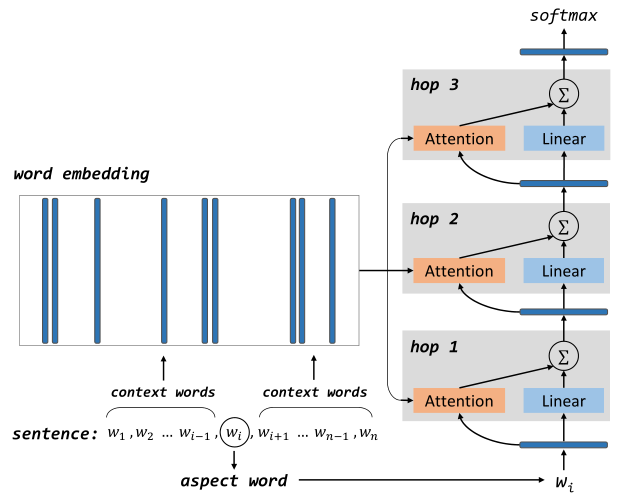
\includegraphics[width=0.7\textwidth]{./figures/tang_memory_network.png}
    \caption{The deep memory network approach for targeted sentiment analysis, with 3 hops. The model stored the context of a target in memory and repeatedly attends to that memory with respect to the target word $w_i$. \cite{tang2016}}
    \label{fig:tang_memory_network}
\end{figure}

\subsection{What are some targeted sentiment analysis approaches that use memory networks?}
Memory networks were first put forward towards the goal of targeted sentiment analysis by \cite{tang2016} (figure \ref{fig:tang_memory_network}). Their approach was inspired by \cite{sukhbaatar2015}, with some differences in the attention function that was used, opting instead to use the method put forward in \cite{bahdanau2014}. The authors reported results outperforming the state-of-the-art SVM-based model by \cite{kiritchenko}, which required extensive manual feature engineering, absent from their proposed memory network, as well as the far more complex LSTM based models \cite{tang2016} which required substantially more time to train. Similar to \cite{sukhbaatar2015}, the authors noted a marginal increase in performance as they increased the number of computational hops, which capped at around 8 hops. 

\cite{chen2017} construct a location-weighted memory module from the hidden states of a BLSTM placed between the input and the attention modules so as to better capture information from phrases comprising of multiple words, such as \enquote{not wonderful enough}. Moreover, unlike the \cite{tang2016}, they combine the results of their recurrent attention layers non-linearly. These improvements led to a performance boost over \cite{tang2016}. The proposed model architecture is illustrated in figure \ref{fig:chen_recurrent_attention_model}. It is also worth pointing out that the authors failed to reproduce the results originally cited in \cite{tang2016}. 

\begin{figure}[!ht]
    \centering
    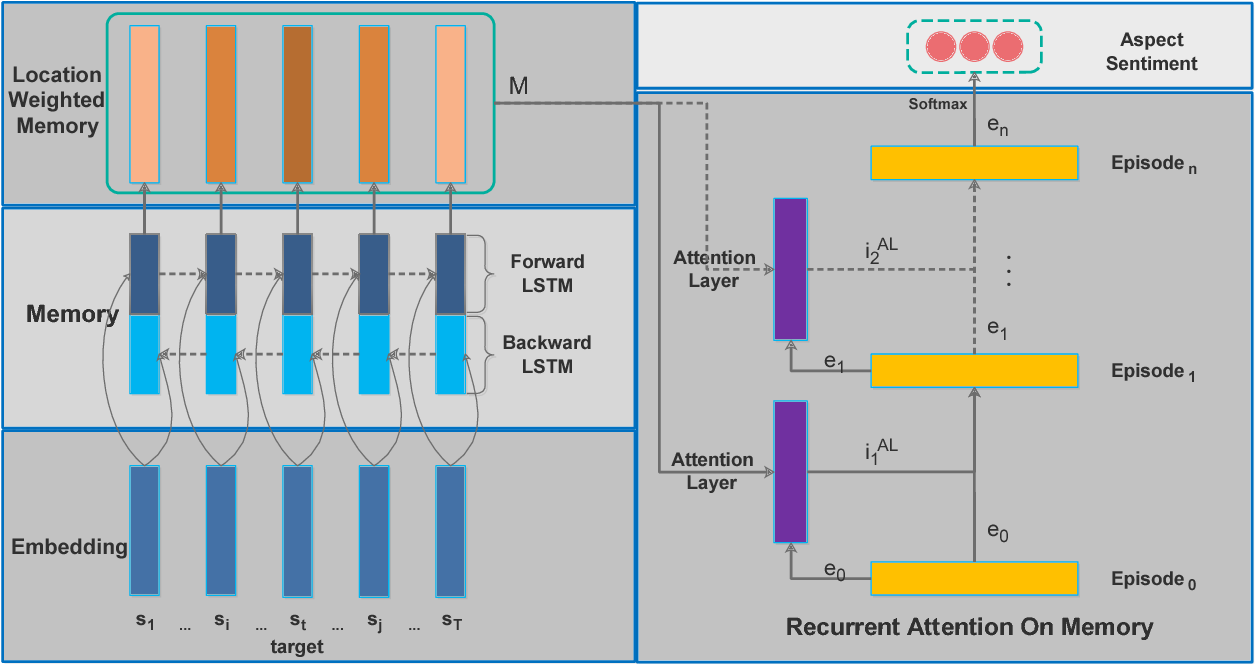
\includegraphics[width=0.7\textwidth]{./figures/chen_recurrent_attention.png}
    \caption{The recurrent attention model architecture showing the placement of the location-weighted memory module with respect to the input and attention layers. As opposed to \cite{tang2016}, the attention values are combined from one episode to the next non-linearly, using a GRU. \cite{chen2017}}
    \label{fig:chen_recurrent_attention_model}
\end{figure}

\cite{liu2018} maintain a memory chain of entities that are encountered while processing a phrase and develop a gating mechanism that determines how those memory chains should be updated. The gating mechanism accounts for the content and the location of the memory chains compared to the current input, as well as the past activations, through the use of a GRU unit, when choosing to update a particular memory element.

\subsection{Why is it imperative to attend to targets as well as contexts?}
Recently, work carried out by \cite{wang2018} showed an interesting performance boundary on approaches to targeted sentiment analysis that make use of attention mechanisms. In particular, \cite{wang2018} note that when context words have diametrically opposing sentimental bearings based on the target being considered, this cannot be modelled by improving by attending to the context alone. 

To illustrate this, \cite{wang2018} consider two different targets, \textit{price} and \textit{resolution}, in four different phrases; \enquote{high price}, \enquote{low resolution}, \enquote{high resolution} and, \enquote{high price}. Some sentiment score, $s$, for these phrases, where $s < 0$ implies a negative sentiment and $s > 0$ implies a positive sentiment accordingly (eq. \ref{eq:sentiment_score}). The attention weight $\alpha$ will have a value of 1 since the context consists of a single word which is represented by $h$. $v$ represents the target and $W$ is the weight matrix the model must learn. 

\begin{equation} \label{eq:sentiment_score}
    s = W(\sum_{i=1}^{n}\alpha_{i}h_{i}+v) = W(h+v)
\end{equation}

From equation \ref{eq:sentiment_score}, the following inequalities can be obtained,
\begin{equation*}
\begin{split}
    W(h_{high}+v_{price}) < 0 \\
    W(h_{low}+v_{price}) > 0 \\
    W(h_{high}+v_{resolution}) > 0 \\
    W(h_{low}+v_{resolution}) < 0
\end{split}
\end{equation*}
Expanding these inequalities results in $Wh_{high}<Wh_{low}<Wh_{high}$, which is a contradiction, and can therefore not be learned by the model. \cite{wang2018} point out that this condition cannot be rectified through further attending to the context but rather ameliorating the representation of the targets $v$ to better capture the complex relationship they have with the context in a way that possibly reverses the polarity of the final sentiment score $s$.

Towards this end, \cite{wang2018} experiment using a series of techniques, and note an improvement over previously cited results as well as a direct improvement on the RAM model \cite{chen2017} when these are coupled with their optimally performing target-sensitive context modelling strategy.

\section{Out-of-vocabulary Words}
\subsection{What are OOV words?}
A common theme in the deep learning models that have been discussed herein is the uncanny similarity between the techniques that these models employ to understand information and the same techniques that the human brain takes advantage of, both consciously and unconsciously, to produce an understanding of the information it is presented, with respect to a particular goal. 

Traits such as properly identifying the most important and informative elements of a sequence, and referring to past events when making such decisions as well the fundamental process by which the intricacies of the networks are tuned when errors are made in training, in an effort to lessen such errors in the future. 

In this analogy, when dealing with language-related tasks such as targeted sentiment analysis, the word embedding matrix from which different words' are represented numerically can be regarded as the working vocabulary that the model has prior to tackling the task at hand.

It stands to reason that due to the ever changing and ever evolving nature of language, it is impossible to account for the entire vocabulary of a particular language when constructing word embeddings. Regardless of the amount of text that is initially used to construct the word embeddings there shall be words that are not encountered within that text and therefore a continuous vector representation of that word could not be produced. While the probability of covering the most commonly occurring words increases with the size of the original text and the variety within it, encountering new words is an inescapable eventuality. These previously unseen words are consequently referred to as out-of-vocabulary (OOV) words. 

The magnitude of the challenge that OOV words present, and the potential repercussions thereof, become evident in the landscape of this analogy. These represent words which the models essentially have no understanding of and can be of little help to it when attempting to extract any information it may convey to the task at hand. While the model can be expected to learn more about these words through repeated encounters in different contexts, the fact that these words, by their own nature, tend to occur infrequently in language substantially diminishes the efficacy of this learning process. 

\subsection{What problems for generative tasks do OOV words create?}
OOV words are of particular concern when dealing with tasks that are generative in nature, such as ASR. The toll of OOV words on the performance of approaches to these tasks is two-fold. Firstly, OOV word may be substituted with an incorrect IV word. Secondly, the OOV word has a direct effect on the neighbouring IV words \cite{naptali2012}.

A common approach to this problem is clustering OOV words into groups that would are sufficiently expressive of their constituents. Various techniques have been employed towards this goal such syntactic and morphological features, part-of-speech tag information, online resources, and subword-level models to name a few, \cite{naptali2012} does a good job of outlining these approaches. 

\subsection{What problems for sentiment analysis do OOV words create?}
Since sentiment analysis is classification task, where words are provided as input and subsequently used as keys when looking up the relevant embedding vector, substituting an OOV word for an IV word is of no concern. The effect of an OOV word on its neighboring words, however, is prone to undermine a model's ability to generate an accurate representation of the content as a whole. 

This sort of phenomenon is not particularly difficult to imagine since it is often times the case in languages that a single word can have drastic effects on the meaning of a phrase, particularly in situations expressing negation. Consider a phrase such as \enquote{It avoids all the predictability found in Hollywood movies.}, where \enquote{predictability} conveys a negative sentiment, which is subsequently negated by the verb \enquote{avoids}.

Moreover, OOV words obviously make the process of comprehending a phrase more difficult by introducing elements that the model has no knowledge of. If the word embedding model that is being used is analogous to the model's understanding of a language, an OOV word is effectively a word the model does not understand, and therefore has limited means by which to gauge the effect of that word on the overall sentiment of the phrase, if any.

\subsection{How are OOV words typically regarded in Sentiment Analysis?}
A typical approach to this OOV challenge within the field of sentiment analysis is the use of a particular singular token that is meant to represent low frequency words during the training phase, and subsequently model all OOV words encountered in the test phase. The vector for this token is often times initialized using some bounded random uniform distribution.

\subsection{Why is this sub-optimal?}
As far back as \cite{gallwitz1996}, before the popularity of pre-trained word embeddings such as \textit{GloVe} and \textit{Word2Vec}, it was pointed out that using a single token is somewhat crude. It could not possibly encompass the wealth of linguistic information expressed by every OOV word that is encountered; consider that an OOV word can be anything from a spelling mistake to proper noun, such as the name of an entity, and anything in between.  

When training an n-gram model, the use of a single \unk label for all OOV words will lead to a substantial inconsistency in the frequency of OOV words between training and test datasets \cite{gallwitz1996}. This inconsistency is comparable to the possibly counter productive training that is carried out on the singular \unk vector across different samples within the scope of sentiment analysis and word embeddings.

In their work, dealing particularly with OOV tokens within the field of Reading Comprehension (RC), \cite{bhuwandhingra2017} note a considerable drop in performance when taking this approach in some cases and suggest that a unique OOV token would lack the desired level of detail to correctly generate a correct answer. 

\subsection{Why are classes better for handling OOV words?}
It is not necessarily useful to approach the OOV word challenge at the word-level. It is assumed that OOV words are scarce, which substantially limits the occasions for a prospective model to learn any discerning information about that word. Attempting to model clusters of OOV words instead, would benefit each member of the cluster by the accumulated frequency of all members \cite{naptali2012}.

Moreover, within the scope of sentiment analysis, the intuition for clustering words under classes characterized by some particular sentimental value, or a lack thereof; as in the case of registered trademarks, would be evidently beneficial.

\subsection{What is the trade-off between too many and too few classes?}
Too few classes may not possess a sufficiently fine level of detail in their discerning characteristics and cluster together words which are unrelated and subsequently erroneously trained together. This can be seen from the extreme of this case, where only a single token is used, and the issues that have been reported for this approach.

Conversely, if an excessive number of classes are used, this would naturally decrease the amount of OOV words within each class, and consequently the frequency of words appearing in a particular sample. This hinders a model's ability to learn any distinguishing characteristics of a class. Taken to the extreme, if each class were to contain only a single word, this would effectively render each class as a randomly initialized vector for this word which is rarely encountered, and trained. This undermines the purpose of a word vector, which is to convey as much information about the word as possible. 

\subsection{Why do i think there are benefits to be had from better OOV handling in SA?}
Within the scope of a RC task, \cite{bhuwandhingra2017}, carry out a study to accurately measure the effects that different embeddings and OOV approaches can have on the final result of two benchmark models. 

They outline the typical approach to RC problems as initially generating a representation of the source document, possibly through the use of pre-trained word embeddings such as \textit{GloVe} in conjunction with statistical models such as the LSTM \cite{hochreiter1997} which may employ an attention mechanism (eg. \cite{bahdanau2014}). The result of this process is a contextual representation of the document from which a valid answer can be extracted. 

It is worth noting that this process is not dissimilar from the majority of approaches that have been adopted recently within the field of sentiment analysis. Both employ similar techniques and maintain the same characteristic order of events in generating a substantive representation of the source, differing only in the objective and hence the final product to be extracted from that representation. While this is by no means an insignificant difference, on a macro level this can be seen merely as adjusting the variables and parameters that are input to the system, as opposed to the system as a whole. 

In their work, \cite{bhuwandhingra2017} suggest that there are notable effects on the downstream results of models when comparing the use of different word embeddings, pre-trained or otherwise. Specifically, as an out-of-the-box solution, they recommend the use of GloVe \cite{pennington} 200-dimension pre-trained embeddings. Moreover, for their benchmark RC models, they recommend assigning random unique vectors for OOV tokens at test time, possibly due to the fact that subjects in generated responses are likely to be OOV token and proper nouns. 

Based on these findings, the aforementioned similarity in the process of tackling RC tasks and SA tasks, along with the challenges that OOV words pose in the field of SA as previously outlined, the study of word embedding choice and OOV approaches and their effects therein is something that we believe merits further investigation.  

\section{Reproducibility}
\subsection{What is reproducibility and why is it important?}
The ability to reproduce experiments is the integral basis upon which all disciplines of science are founded. Within many fields, NLP among them, this typically entails adherence to three integral guidelines, namely, (a) the provision of sufficiently detailed methodologies, (b) the release of operational code-bases and (c) access to the dataset(s) with clear details pertaining to any processing and/or stratification strategies used. These guidelines ensure that results can be easily reproduced, evaluated for generalizability and compared to other methods in the field, thereby fostering growth. 

\subsection{What is the state of reproducibility in the field of Targeted sentiment analysis?}
In \cite{moore2018}, the authors underscore the significance of reproducibility of approaches as well as the generalizability of the results that are reported, and proceed to argue that adherence to the aforementioned tenets has been lacking in recent years, paying particular attention in their work to the field of targeted sentiment analysis. 

The authors also draw attention to the fact that a multitude of studies report results on different datasets which often stem from diverse sources that could be composed of language that is centered around a particular topic. Notable still, these datasets also exhibit consequential statistical differences such as the average length of, and/or amount of targets in, a sentence. Occasionally, studies also carry out particular alterations to existing datasets or adopt a specific strategy for merging one or more datasets (eg. \cite{xue2018}). These factors substantially limit the possibility of effectively comparing the novel approaches as they emerge in the field.  

Replication studies such as \cite{moore2018} can remedy this issue by attempting to reproduce the studies in a comparative setting, however they outline challenges in this regard as well. The authors note that a number of approaches in the field fail to outline the precise pre-processing steps they adopted, which may have substantial effects on the downstream performance of a model, and thus make reproducing the results difficult. In some situations they also note model settings mentioned that are not necessarily self-evident, such as a "softmax clipping threshold" \cite{tang2016b}, which, in attempting to reproduce the study, \cite{moore2018} were forced to ignore as they were unfamiliar with the term. 

One key observation that \cite{moore2018} also make with regards to deep learning and neural network based approaches such as \cite{tang2016b} is the influence that an initial random seed has on the final performance results, particularly when using smaller word embeddings (\cite{reimers2017} as cited in \cite{moore2018}). They mention this as the probable reason for other studies \cite{chen2017},\cite{tay2017} (including their own), not being able to recreate the original results reported in \cite{tang2016b}. The authors remark that in situations such as this, when dealing with models of this nature, it would be well-advised to gauge a model's performance over a number of experiment runs as opposed to one.

\section{Objectives}
Following the principles outlined in \cite{moore2018}, and motivated by the observations made by \cite{bhuwandhingra2017} in the field of reading comprehension and the effect of OOV embedding strategies thereof, the objectives of this study are two-fold.

\begin{enumerate}
    \item We intend to extend the work carried out by \cite{moore2018} in the field of TSA to cover a wider range of studies, including those that employ techniques that have since emerged focusing on attention mechanisms and memory networks. This entails the attempt to reproduce these models based on the detail provided in the original studies and subsequently carrying out a comparative evaluation of these approaches across a wide range of datasets from varying domains using a number of different pre-trained word embeddings.
    \item Inspired by the work and findings of \cite{bhuwandhingra2017}, we shall endeavor to investigate the effect that different OOV embedding strategies and pre-trained word embeddings have on the downstream performance of models with respect to TSA. To our knowledge, at the time of writing, this study will be the first to investigate this issue in detail.
\end{enumerate}

To achieve these goals, we make three principal contributions through this work:
\begin{itemize}
    \item A publicly accessible framework that provides access to a range of frequently cited datasets that have been used in the field of TSA. This framework shall be used to obtain robust performance metrics, such as macro-f1 scores for all models, which have been hitherto unreported for a subset of the models, as well as other informative measures that shed light into the inner workings of the models implemented, where applicable (such as attention heat-maps). 
    \item A comparative evaluation of models across different domains and datasets, using different pre-trained word embeddings to ascertain the degree to which results obtained are reproducible and generalizable. 
    \item Detailed reports on a series of experiments using different OOV embedding strategies, across all implemented models, the results of which will allow us to deduce the degree to which these affect downstream performance and whether an optimal approach can be found that proves to be generally beneficial. 
\end{itemize}

Finally, the proposed framework shall also serve as groundwork for future experimentation into alternative, more sophisticated, OOV embedding approaches while also providing a means of rapidly carrying out comparative evaluations of TSA models across different datasets and pre-trained word embeddings.  


\chapter{Design}
% A detailed explanation of how the problem was tackled along with justifications for all decisions taken in the course of the solution.

% Design chapter Intro
%     describe the conceptual design of the framework  
%     provides reasons for notable design choices made
%     Show image of the block diagram
%     Next sections cover design details of the Data and Experiment module, and their constituent components
%     Specific implementation details are given in chapter 4 
%     Chapter 5 describes the evaluation measures produced by the framework
    

\section{Data Module}
The primary task of the data module is to produce the features data for the experiment module. We sought to adopt a modular design paradigm since this allows different responsibilities to be delegated to the appropriate sub-component. 

Each sub-component of the data module is responsible for writing and indexing data to an external file-system using a specific hashing policy when this data is first generated. In subsequent experiments that require this same data, the sub-component is tasked with querying the file-system for its availability and importing it, instead of having to reproduce it. 

Maintaining this indexed data store on the external file-system has the benefits of speeding up computation for subsequent experiments that use the same data with parametric alterations, facilitating investigation of the data produced at intermediary steps, aiding in debugging and allowing the framework to isolate the minimum requirement of data that to upload for experiments carried out through online services. 

\subsection{Dataset Import Script}
It is imperative to evaluate the performance of TSA models on datasets that have different characteristics, as a measure of the applicability of the model under different scenarios, or for the purposes of fine-tuning a model to a specific domain. Datasets from different platforms and domains vary in their vocabulary and other vernacular features, such as colloquialisms. Different platforms also provide samples of varying lengths and which may express different sentiments towards multiple targets in the same sample. 

\subsubsection{Raw Data Parsing Function}
The import script simplifies the process of importing new datasets to only requiring a, typically short, parsing function which reads the raw data files and mutates the data structure to records consisting of four fields: sentence, target, sentiment label and, offset\footnote{required to identify the correct target in situations where it occurs more than once in the same sentence}. The parsing function is an inevitable requirement since it is unfeasible to account for all the possible data formats of prospective datasets, the specifics of this function are explained in [\S4: Parsing Function]. 

Once imported, the dataset is stored and indexed on the file-system for future use under a user-defined name. The imported data is stored in two dictionaries, for training and testing, and exported as binary pickle\footnote{python serialized object file} files, which provides the fastest access times at minimal storage cost. 

\subsection{Dataset Component}
The dataset component is primarily tasked with loading dataset files which have been imported as well as generating the accompanying information files used at other points in the process. Moreover, the component is also responsible for creating and exporting re-distributed variants of datasets, serving as a wrapper around these operations with which other sub-components in the data module can interact. 

The corpus file that is generated by the dataset component provides a record of the occurrence count of each unique term in the dataset and is subsequently used to filter the vocabulary of an embedding to the minimal set of required terms. The \textit{.json} file that is generated provides information on the distribution of the dataset, later used by the experiment component in producing a visual representation of this information. Two variants of each file are created, for the training and testing subsets of the dataset respectively.

\subsubsection{Dataset Re-Distribution}
It is often the case in datasets typically employed for TSA that one or more sentiment labels are over-represented in the data, indeed, this phenomenon is common across all the datasets gathered for this work. This is accounted for at the output stage by using appropriately weighted performance metrics, as detailed in \S5. 

This notwithstanding, such an imbalance in classes causes the model to be overexposed to a particular sentiment at the cost of others, which may be detrimental to the learning process. To address this issue, while also providing a means of investigating the effects of these imbalances, the framework provides a means of re-sampling the data, either to balance the distribution across all classes, or to any custom distribution as specified by the user.

The implementation details of the algorithm developed for this purpose are provided in [\S4: Dataset re-distribution].

\subsection{Embedding Component}
As with the dataset component, the goal of the embedding component is to provide a wrapper around reading and writing to and from an indexed embeddings directory by specifying a singular embedding type that exposes all the required data to allow the other sub-components to interact with it, facilitating the integration of additional embedding sources later in the development stage. 

The commonly used embeddings are identified using a pre-defined shorthand, which the embedding component takes as input, along with a comma-delimited list of filters to apply on the embedding vocabulary. Function filters are specified using a custom name that is assigned when creating the filter. The \enquote{corpus} keyword is reserved within this scope and applies a set filter on the embedding vocabulary using the corpus of the datasets being used for the experiment. The embedding variable is initially obtained using the \textit{GenSim} tool, which provides a means to download some commonly used embeddings. Once the embeddings are downloaded, the data files are stored and indexed within the embeddings directory of the framework, enabling offline access.

\subsubsection{Filtering Embeddings}
If one or more filters are specified, the embedding component extracts the vocabulary of the source embedding, unifies the requested filters into a single pipeline, runs the source vocabulary through this pipeline, and finally re-constructs the embedding on this filtered vocabulary. The resulting data is exported and indexed, along with a JSON file with the details of the filtration process and, in the case of function filters, a CSV report detailing which terms were filtered and what condition was met that resulted in this term being filtered.

The first type of filters that the embedding component supports are set filters, which simply define the set of terms to include from the entire embedding vocabulary. These filters are primarily used to limit the size of the embedding to contain only terms that occur in a dataset corpus, substantially reducing the file-size overhead of the embedding. The other type of filters that are supported are function filters, which refer to a function that, for each term, returns true or false as to whether to keep or discard it. These filters can be used to remove vocabulary terms based on particular POS tags and were implemented in an effort to investigate additional methods of reducing embedding sizes with a minimal cost to downstream performance. 

Processing an entire embedding vocabulary to obtain NLP tags can be significantly time-consuming due to the size of these vocabularies. In an effort to optimize this process, a base function filter is implemented from which an end-user extends, to construct custom function filters. This base class automatically exposes the NLP attributes requested by the user while also allowing the framework to gather all filters into a singular pipeline, used to determine the minimum amount of processing needed to obtain the attributes that this pipeline requires. The implementation details of this procedure are detailed in [\S4: embedding filters].

In order to run multiple experiments using cloud computing services, all of the required data for these experiments need to be uploaded for each job. Apart from maximizing the ability to share data between experiments, reducing redundancy, the final size footprint of this data needs to be minimized to obtain feasible upload times. Since embedding variables were the largest bottleneck in this regard, set filters were used to reduce the size of embeddings to the bare necessity. Although the full embedding vocabulary would still be used at a production level, this reduction in embedding size also provided a marked speedup in look-up operations when indexing datasets, since the size of the look-up table was drastically reduced, resulting in faster experimentation times during development. Function filters were developed as an exploration of other techniques for further size reduction and their effect on downstream performance. The intuition behind this is that the contribution of subsets of vocabulary, such as adjectives and nouns, would suffice within the scope of TSA.

It is essential that the filtering mechanism be intuitive so as to enable extensibility by the end user. The framework grants access to NLP attributes of each particular term within the scope of a function filter. This design allows for a simple means of constructing custom filters that can operate on POS tags and other language characteristics without the need of manually extracting this information from the vocabulary.

Filtered versions of an embedding are stored under a single directory based on the source embedding from which the filter originated. Indexing these directories using a unique hash that is generated from the filter specification enables the embedding component to load a filtered embedding using its hash identifier if it already exists.

\subsection{Feature Provider Component}
The feature provider is detached from the other components of the data module as it is responsible for generating data that is mostly conditional on the specific experiment being carried out, which limits its re-usability, unlike the dataset and embedding components. Aside from managing an indexed directory of this data, the feature provider is primarily responsible for producing both the feature data and number of auxiliary files. The purpose of the latter includes saving the state of data at different stages of the process, providing valuable information used when creating some of the output visualizations, as well as logging diagnostics on the process, for debugging and profiling purposes.

The steps that the feature provider takes to generate the required features are as follows: first, in the case of multiple datasets, these are merged and encompassing corpora are constructed for training and testing, second, text pre-processing and tokenization are carried out producing string tokens to be mapped to integer indices. A look-up-table is finally constructed from the vocabulary of the embedding and a TensorFlow graph of look-up operations is built to map these tokens to their respective indices within the embedding. Upon completion, the results of the graph are converted and exported into a proprietary TensorFlow Record (\textit{TFRecord}) format to be consumed by the experiment module.

As inputs, this component requires an embedding object, one or more dataset objects, and the specific OOV policy that is to be adopted when constructing mapping tokens into features for the experiment module. The indices mapped to each token are contingent on whether OOV tokens are considered at all, solely during training, or whether a particular bucketing strategy is used. If OOV tokens are ignored, this needs to be addressed at the tokenization stage by excluding these tokens. In the case where OOV tokens are only considered at the training stage, the process is similar, excluding only OOV tokens found in the test data, whereas when using a bucketing strategy, no tokens are excluded, and the mapping process is handled accordingly by the look-up table operation. Moreover, the mapped values for OOV tokens vary based on the OOV policy that is adopted, including the number of OOV buckets that are used, since this directly alters the hashing function that assigns the bucket to each token. All of these factors are taken into consideration and handled internally by the framework's own hashing mechanism, creating new data when required and re-using any computationally expensive data where possible.

Although trivially simple, the mapping process can becomes increasingly time-consuming for larger look-up tables, as the look-up ops would be required to traverse more data as a consequence. The initial approach to the problem was to optimize the python code responsible, through the use of generators and parallel processing libraries. These benefits from this approach were quickly exhausted however, and the approach proved to be unreliable, requiring fine-tuning based on the nature of the data being processed. To address this, the process was instead implemented using TensorFlow itself which is particularly adept at optimizing parallelizable operations by first expressing them in graph form, and subsequently executing handling resources and parallelizing operations wherever possible during graph execution, providing more consistent performance. Furthermore, the framework also generates a \textit{filtered} vocabulary file containing only the tokens that occur in the datasets being used, and their corresponding index in the larger embedding vocabulary which is used for building a look-up table at a fraction of the size of the original embedding vocabulary, for the exclusive purpose of mapping the tokenized datasets being considered.

\subsubsection{Merging Datasets}
As previously alluded to, different datasets are characterized by the different attributes and vocabulary that they provide based on the limitations of the platform from which they are sourced, such as the character limit on Twitter, or a specific domain around which they center, such as reviews of a specific type of product. A mechanism by which these datasets could be merged allows us to capture a wider range of these characteristics in both training and testing data and evaluate the performance of different TSA approaches across these variances.

\subsubsection{Text Pre-Processing}
Spacy\footnote{Public NLP library for python, accessible through https://spacy.io/} was used for all text-processing and tokenization tasks. One of the primary reasons for using this tool was its native and intuitive support for parallelization. Secondly, its proprietary language model format enables selectively loading sub-modules based on run-time requirements, improving performance by avoiding superfluous processing. 

Text normalization is kept to a minimum since the exploration of these techniques is beyond the scope of this work. First, for embeddings with case-insensitive vocabularies, all tokens are lower-cased accordingly. Furthermore, a default filter function is implemented which omits URLs and email addresses, and which is detached from the feature provider, facilitating extensibility by the end user.

\subsubsection{Output Data}
The most salient outputs of the feature provider are the \textit{TFRecord} files containing the feature data for the experiment module. These features are exported to separate directories for training and testing data and further partitioned, following TensorFlow guidelines for ensuring integrity when batching and randomizing this data through their data pipeline API. Other important outputs of the feature provider are the vocabulary files that can be used to visualize the embedding using TensorBoard and a JSON reference file detailing the datasets and embeddings as well as OOV policy employed. The latter includes details on the OOV initialization function and a list of the OOV buckets and their constituent tokens, providing insights into the behavior of the bucketing function\footnote{by default is a hashing function handled internally by TensorFlow}.

Finally, similar to other components, data at multiple stages are exported to pickle files for two reasons. Firstly, this foregoes the need for carrying out repetitive processing. Secondly, by loading these files at different stages of the feature generation process in an online setting, where computationally expensive tasks are kept to a minimum, the feature provider can maintain its internal state, preserving the value of all of its class members. Indeed, this is desired for all components; maintaining an identical internal state in both offline and online environments reduces the risk of costly online experiment failures resulting from run-time errors.

\chapter{Implementation}
\section{Importing Datasets}
The framework provides a CLI command as an entry point for importing new datasets. The command signature requires a path to a directory containing three files at a minimum: a \enquote{train} and \enquote{test} file and an accompanying parser Python\footnote{Python3 syntax is expected} script. This API additionally exposes arguments for specifying a custom identified under which to index the imported data, as well as a specific parser in situations where multiple parsers are provided.

The parsing script will typically consist of two stages: reading and mutating the raw data. The first is contingent on the format of the raw data being imported and can vary in complexity from simply reading from a text file to more complex operations on proprietary data formats. The second stage generally involves the use of generators and looping structures to iterate through raw samples and produce the arrays the framework expects. This stage also presents an opportunity for the user to incorporate any conditional filtering or transformations, such as excluding \enquote{conflict} labels from raw datasets. The function must produce three arrays consisting of the sentences, targets, and labels. A fourth array, of character offsets of each target, may also be returned. This is optional for datasets where each target appears only once in each sentence, but required otherwise, as the framework would have no means of differentiating between multiple target occurrences in a sentence.

The signature that is enforced by the framework on the parsing function stipulates that it expects solely one parameter without a default value, which is reserved for the path of the file to be parsed. For most cases a single function will suffice, however in some instances, multiple functions may be required for improved  separation of concerns. In these situations, both the parsing script and the function that serves as the primary entry point within it must be named according to the provided \texttt{parser-name} CLI argument.

Initially, the framework scans the directory for the relevant source files which contain the words \enquote{test} and \enquote{train} in their names. The parsing script is loaded based on the provided parser name argument or the default parser file-name. Once all required files are located, the framework inspects the parsing script and ensures that the parsing function has the expected signature. Provided all these tests are passed, the framework proceeds to run the parsing script on the raw data then stores the result in its own hashed index of datasets under the user-provided identifier for future use.

This mechanism for importing datasets provides the widest range for support of various data types while maximally extrapolating the code responsible for this operation, thereby simplifying the process for the end-user. Furthermore, the framework is abstracted from the dataset importing process thereby limiting the scope of errors that may occur during the process to the parsing script itself, which is easier to debug by the end-user as opposed to the internal code of the framework. 

Finally, the structure of this approach allows for the possibility of defining multiple parsing functions, each of which may carry out processing or filtering operations prior to importing the dataset, while also delegating the responsibility of storing and accessing these different versions of a dataset to the framework.

\section{Dataset Re-Distribution}
\begin{algorithm}[H]
\SetAlgoLined
\KwData{Previous Class Label Counts, Target Class Label Distribution}
  \KwResult{New Class Label Counts}
  initialization\;
  \While{not at end of this document}{
    read current\;
    \eIf{understand}{
      go to next section\;
      current section becomes this one\;
    }{
      go back to the beginning of current section\;
    }
  }
\caption{Dataset Re-Distribution Algorithm}
\end{algorithm}

\section{Datasets}
The following section presents a brief overview of the datasets that were chosen to be integrated into the framework. We focus on the principal factors that were considered when choosing these datasets with the intention of maximizing the diversity in these attributes. These include the mechanism by which the datasets where originally obtained and annotated, the respective platform from where they were sourced, any specific domain around which they center and finally we present any salient statistical information that characterizes the datasets.

\subsection{Dong Twitter Dataset}
\cite{dong} is one of the most frequently cited datasets for TSA, used in works such as \cite{tang2016b}, \cite{chen2017} and \cite{zheng2018}. This dataset comprises tweets focusing on a diverse range of topics that were obtained through the twitter streaming API by querying for targets such as \enquote{bill gates} and \enquote{xbox}. This implies that, in each instance, the target string occurs explicitly in the tweet. The respective sentiment of each tweet towards its target is manually annotated as \enquote{positive}, \enquote{neutral} or \enquote{negative}, and the authors report a fair inter-annotator agreement score of $0.82$.  The final dataset consists of 6248 training samples and 692 testing samples, each having a distribution consisting of twice as many neutral samples as positive and negative combined. As some studies \cite{wang2017} \cite{saeidi2016} that followed point out, a notable property of this dataset is the fact that each sample is restricted to having a single target. It is worth noting that due to the skewed nature of the class distribution, it is imperative that a metric that accounts for this is reported, such as the Macro-F1, when evaluating performance on this dataset.

\subsection{Saeidi Yahoo Answers Dataset}
In their work, \cite{saeidi2016} combine the tasks of detecting the existence of a particular aspect as well as the sentiment with respect to that aspect within pieces of text obtained from \enquote{Yahoo! Answers} concerning specific neighborhoods in or around the city of London. The authors suggest that this text tends to be less constrained than that originating from social media platforms, and that this enables them to obtain reviews that mention multiple neighborhoods per instance with differing sentiments. The final dataset is limited to samples that contain up to two targets and these are manually annotated using binary labels (\enquote{positive} and \enquote{negative}) across eleven separate aspects such as \enquote{dining} and \enquote{shopping}. These aspects do not necessarily occur within the text itself and are therefore inconsequential within the scope of TSA. This notwithstanding, a \enquote{general} aspect category is also considered, used to denote a \textit{general} sentiment towards a particular entity or target, and is the most frequently annotated category. We consider only this subset of samples from this dataset and only use the train and test portions, discarding the development portion. It is important to note that all original target mentions within this dataset are obfuscated through the use of "location markers" thereby eliminating any additional context information that could be conveyed by the target itself. The final datasets consists of 1770 sentences, 78\% of which are labelled positive. To the best of our knowledge, the baselines implemented in this work have not previously been evaluated on this data. 

\subsection{Wang Political Twitter Dataset}
A point that \cite{saeidi2016} stresses on in developing their dataset is the importance of considering an approach's ability to discern different and possibly opposing sentences towards multiple targets in the same phrase. With this same goal in mind, \cite{wang2017} build a dataset consisting of tweets centered around UK politics, labelled according to the sentiment expressed towards a specific target entity that occurs in the tweet, using a 3-point scale. Across 4077 tweets, a total of 12587 targets are identified with just under half (6015) of those expressing a negative sentiment and an average of 3.09 targets per sentence. As pointed out in \cite{moore2018}, there are a number of samples in this dataset where the target locations are not specified, which makes tweets where the target occurs more than once unusable since there is no way of knowing which instance is being considered. We exclude these cases for our experiments, resulting in a reduced dataset which contains 11899 target-sentiment pairs in total; with 2190 unique targets and an average of 2.94 targets per tweet. 

\subsection{SemEval Laptop \& Restaurant Reviews Dataset}
Another dataset commonly cited in the field of targeted sentiment analysis and aspect-based sentiment analysis is the Restaurant and Laptop Reviews dataset \cite{pontiki}. This dataset comprises of a total of 7686 sentences from two distinct domains, namely technology and dining, from which specific aspect terms and the respective polarity towards them were manually annotated. Sentiment polarity was determined on a 3 point scale with the addition of a \enquote{conflict} label which we do not consider in our experiments. Compared to data sourced from micro-text platforms the samples in this dataset are typically lengthier and more syntactically sound. The authors note some interesting differences in the nature of the reviews obtained from the two domains such as the restaurant subset containing substantially more aspect terms and a stronger bias towards the positive sentiment compared to the laptop reviews. The majority of targets in both domains consist of a single word. Recently, \cite{xue2018} used this dataset for their evaluation purposed and included results for three of the five baselines implemented in our work, namely, IAN \cite{dehongma2017}, RAM \cite{chen2017} and TD-LSTM \cite{tang2016b}. 

\subsection{SemEval 2015 Twitter Dataset}
This dataset was specifically proposed for the task of sentiment analysis on twitter as part of the SemEval challenge \cite{rosenthal2015}. A subset of the dataset which we are interested in within the confines of this study consists of a series of tweets which were collected and manually annotated with a 3-scale sentiment polarity score directed towards a particular entity term occurring in the tweet. The annotation process was carried out using Amazon's Mechanical Turk system with 5 turks, employing a majority vote in cases where an agreement could not be obtained. For the purposes of our study we make use of the training and testing subsets of the dataset and interchange these two subsets so as to have a larger training dataset as opposed to testing set, as in the previous datasets outlined. Moreover, in its original form this dataset consisted only of tweet IDs  from this the original tweet can be obtained however only within a specific window. In out experiments we were able to obtain a  downloaded version of this data, which included the original tweet text, from a later SemEval submission \cite{baziotis2017} from their github repository. The final dataset consists of 2872 samples, the majority of which are labelled \enquote{positive}.

\subsection{SemEval 2016 Twitter Dataset}
Similar to the previously mentioned dataset, this was also constructed for the purposes of the SemEval sentiment analysis on twitter challenge \cite{nakov2016}, with the difference of being graded on a 5-point scale as opposed to a 3-point and also comprising substantially more samples and topics than the former. For the purposes of our work, we reduce the resolution of this dataset from a 5-point scale to a 3-point scale by grouping \enquote{very negative} and \enquote{weakly negative} samples under a single \enquote{negative} label, and similarly for \enquote{very positive} and \enquote{weakly positive}, to obtain \enquote{positive} samples. The annotation process that was employed is similar to that outlined in the \cite{rosenthal2015} with minor differences in the majority voting system for conflict resolution around label disagreements due to the different point-scale (the process is detailed in \cite{nakov2016}). The actual tweet data for this dataset was also obtained from the Github repository of \cite{baziotis2017} due to the same limitation around this data expiring after a particular time-window. The test and train splits of the dataset were similarly interchanged to obtain a larger training dataset. The final dataset includes over 20000 training samples covering 100 topics, with the overwhelming majority being either \enquote{neutral} or \enquote{positive}. Whereas the testing dataset consists of 6000 samples with entirely different topics and is skewed towards the \enquote{positive} label.

\begin{table}[]
\centering
\begin{tabular}{|l|l|l|l|c|c|}
\hline
\multicolumn{1}{|c|}{\textbf{Dataset}} & \multicolumn{1}{c|}{\textbf{Domain}} & \multicolumn{1}{c|}{\textbf{Type}} & \multicolumn{1}{c|}{\textbf{Split}} & \textbf{\begin{tabular}[c]{@{}c@{}}Vocabulary \\ Size\end{tabular}} & \textbf{\begin{tabular}[c]{@{}c@{}}Unique \\ Targets\end{tabular}} \\ \hline\hline
\multirow{3}{*}{Dong}                  & \multirow{3}{*}{General}             & \multirow{3}{*}{Social Media}      & Test                                & 3682                                                                & 82                                                                 \\
                                       &                                      &                                    & Train                               & 15037                                                               & 113                                                                \\ \cline{4-6} 
                                       &                                      &                                    & \textbf{Total}                      & \textbf{16047}                                                      & \textbf{118}                                                       \\ \hline\hline
\multirow{3}{*}{Saeidi}                & \multirow{3}{*}{General}             & \multirow{3}{*}{Review}            & Test                                & 1231                                                                & 2                                                                  \\
                                       &                                      &                                    & Train                               & 1804                                                                & 2                                                                  \\ \cline{4-6} 
                                       &                                      &                                    & \textbf{Total}                      & \textbf{2257}                                                       & \textbf{2}                                                         \\ \hline\hline
\multirow{3}{*}{Wang}                  & \multirow{3}{*}{Politics}            & \multirow{3}{*}{Social Media}      & Test                                & 4385                                                                & 755                                                                \\
                                       &                                      &                                    & Train                               & 9706                                                                & 1855                                                               \\ \cline{4-6} 
                                       &                                      &                                    & \textbf{Total}                      & \textbf{11211}                                                      & \textbf{2190}                                                      \\ \hline\hline
\multirow{3}{*}{Pontiki - R}           & \multirow{3}{*}{Restaurants}         & \multirow{3}{*}{Review}            & Test                                & 1945                                                                & 520                                                                \\
                                       &                                      &                                    & Train                               & 3635                                                                & 1168                                                               \\ \cline{4-6} 
                                       &                                      &                                    & \textbf{Total}                      & \textbf{4292}                                                       & \textbf{1500}                                                      \\ \hline\hline
\multirow{3}{*}{Pontiki - L}           & \multirow{3}{*}{Technology}          & \multirow{3}{*}{Review}            & Test                                & 1408                                                                & 389                                                                \\
                                       &                                      &                                    & Train                               & 3174                                                                & 945                                                                \\ \cline{4-6} 
                                       &                                      &                                    & \textbf{Total}                      & \textbf{3510}                                                       & \textbf{1181}                                                      \\ \hline\hline
\multirow{3}{*}{Rosenthal}             & \multirow{3}{*}{General}             & \multirow{3}{*}{Social Media}      & Test                                & 3243                                                                & 44                                                                 \\
                                       &                                      &                                    & Train                               & 9800                                                                & 137                                                                \\ \cline{4-6} 
                                       &                                      &                                    & \textbf{Total}                      & \textbf{11575}                                                      & \textbf{180}                                                       \\ \hline\hline
\multirow{3}{*}{Nakov}                 & \multirow{3}{*}{General}             & \multirow{3}{*}{Social Media}      & Test                                & 19374                                                               & 60                                                                 \\
                                       &                                      &                                    & Train                               & 43859                                                               & 100                                                                \\ \cline{4-6} 
                                       &                                      &                                    & \textbf{Total}                      & \textbf{54034}                                                      & \textbf{160}                                                       \\ \hline
\end{tabular}
\caption{Dataset domains, vocabulary sizes, and the number of unique targets.}
\label{tab:dataset_domain_vocab}
\end{table}

\begin{table}[]
\centering
\begin{tabular}{|l|ccc|}
\hline
\multicolumn{1}{|c|}{\multirow{2}{*}{\textbf{Dataset}}} & \multicolumn{3}{c|}{\textbf{\begin{tabular}[c]{@{}c@{}}Target Length\\ (tokens)\end{tabular}}} \\ \cline{2-4} 
\multicolumn{1}{|c|}{}                                  & \textbf{1}                    & \textbf{2}                    & \textbf{3+}                    \\ \hline
Dong                                                    & 2080                          & 4851                          & 9                              \\
Saeidi                                                  & 1770                          & 0                             & 0                              \\
Wang                                                    & 9702                          & 1937                          & 260                            \\
Pontiki - R                                             & 4449                          & 977                           & 528                            \\
Pontiki - L                                             & 2143                          & 982                           & 410                            \\
Rosenthal                                               & 1554                          & 1145                          & 170                            \\
Nakov                                                   & 11450                         & 13684                         & 1366                           \\ \hline
\end{tabular}
\caption{Number of targets of different lengths, in tokens.}
\label{tab:dataset_target_length}
\end{table}

\begin{table}[]
\centering
\begin{tabular}{|l|l|c|ccc|}
\hline
\multicolumn{1}{|c|}{\textbf{Dataset}} & \multicolumn{1}{c|}{\textbf{Split}} & \textbf{Samples} & \textbf{Negative} & \textbf{Neutral} & \textbf{Positive} \\ \hline\hline
\multirow{3}{*}{Dong}                  & Test                                & 692              & 173               & 346              & 173               \\
                                       & Train                               & 6248             & 1560              & 3127             & 1561              \\ \cline{2-6} 
                                       & \textbf{Total}                      & \textbf{6940}    & \textbf{1733}     & \textbf{3473}    & \textbf{1734}     \\ \hline\hline
\multirow{3}{*}{Saeidi}                & Test                                & 588              & 139               & -                & 449               \\
                                       & Train                               & 1182             & 246               & -                & 936               \\ \cline{2-6} 
                                       & \textbf{Total}                      & \textbf{1770}    & \textbf{385}      & \textbf{-}       & \textbf{1385}     \\ \hline\hline
\multirow{3}{*}{Wang}                  & Test                                & 2541             & 1206              & 957              & 378               \\
                                       & Train                               & 9358             & 4377              & 3615             & 1366              \\ \cline{2-6} 
                                       & \textbf{Total}                      & \textbf{11899}   & \textbf{5583}     & \textbf{4572}    & \textbf{1744}     \\ \hline\hline
\multirow{3}{*}{Pontiki - R}           & Test                                & 1357             & 258               & 279              & 820               \\
                                       & Train                               & 4597             & 1128              & 926              & 2543              \\ \cline{2-6} 
                                       & \textbf{Total}                      & \textbf{5954}    & \textbf{1386}     & \textbf{1205}    & \textbf{3363}     \\ \hline\hline
\multirow{3}{*}{Pontiki - L}           & Test                                & 743              & 153               & 218              & 372               \\
                                       & Train                               & 2792             & 1013              & 633              & 1146              \\ \cline{2-6} 
                                       & \textbf{Total}                      & \textbf{3535}    & \textbf{1166}     & \textbf{851}     & \textbf{1518}     \\ \hline\hline
\multirow{3}{*}{Rosenthal}             & Test                                & 486              & 56                & 288              & 142               \\
                                       & Train                               & 2383             & 260               & 1256             & 867               \\ \cline{2-6} 
                                       & \textbf{Total}                      & \textbf{2869}    & \textbf{316}      & \textbf{1544}    & \textbf{1009}     \\ \hline\hline
\multirow{3}{*}{Nakov}                 & Test                                & 5868             & 749               & 1623             & 3496              \\
                                       & Train                               & 20632            & 2339              & 10081            & 8212              \\ \cline{2-6} 
                                       & \textbf{Total}                      & \textbf{26500}   & \textbf{3088}     & \textbf{11704}   & \textbf{11708}    \\ \hline
\end{tabular}
\caption{Dataset sizes and class distributions. }
\label{tab:dataset_class_dists}
\end{table}

\begin{table}[]
\centering
\begin{tabular}{|l|c|cc|ccc|}
\hline
\multirow{2}{*}{\textbf{Dataset}} & \multirow{2}{*}{\textbf{\begin{tabular}[c]{@{}c@{}}Average Targets\\ /Sentence\end{tabular}}} & \multicolumn{2}{l|}{\textbf{\begin{tabular}[c]{@{}c@{}}Sentence Length\\ (tokens)\end{tabular}}} & \multicolumn{3}{c|}{\textbf{\begin{tabular}[c]{@{}c@{}}Distinct Sentiments\\ /Sentence\end{tabular}}} \\ \cline{3-7} 
                                  &                                                                                               & \textbf{Average}      & \textbf{/Target}      & \textbf{1}                       & \textbf{2}                      & \textbf{3+}                      \\ \hline
Dong                              & 1                                                                                             & 21.1                  & 21.1                  & 6934                             & 0                               & 0                                \\ 
Saeidi                            & 1.24                                                                                          & 15.2                  & 12.4                  & 1416                             & 23                              & 0                                \\ 
Wang                              & 2.94                                                                                          & 26.3                  & 9                     & 2163                             & 1640                            & 242                              \\ 
Pontiki - R                       & 2.31                                                                                          & 21.4                  & 7.4                   & 2177                             & 379                             & 20                               \\ 
Pontiki - L                       & 1.92                                                                                          & 22.7                  & 10                    & 1665                             & 193                             & 9                                \\ 
Rosenthal                         & 1.01                                                                                          & 23                    & 22.8                  & 2842                             & 5                               & 0                                \\ 
Nakov                             & 1.01                                                                                          & 23.2                  & 23.1                  & 26355                            & 40                              & 0                                \\ \hline
\end{tabular}
\caption{Dataset sentence information}
\label{tab:dataset_sentence_info}
\end{table}

% \begin{proof}
% this is a proof
% \end{proof}

\chapter{Evaluation}
% Details about how the solution was evaluated with respect to the original research question(s) along with the results achieved.
% \section{Datasets}
% \subsection{Reviews}
% SemEval restaurant and laptop dataset \cite{pontiki}.\\
% \subsection{Social Media}
% Social media datasets are provided in \cite{socher2013}, \cite{dong}, \cite{pontikib} and \cite{saeidi2016}.\\

\section{Evaluation Metrics}

\chapter{Results and Observations}



\chapter{Conclusion}
% An outline of the main conclusions from the student’s research an the impact of these conclusions on the field.
\section{Future Work}
% Proposals for the student him/herself or other future researchers with regards to how the work can be extended or used as a basis for future work in the are.
\appendix

\chapter{Appendix A}
\section{These are some details}
%%example of the code environment
\begin{code}
this is some code;
Make sure to use this template.
\end{code}


\bibliomatter



\bibliographystyle{abbrv}
 \bibliography{references}
 
\end{document}
